\chapter{Base de datos} 
\label{section_base_de_datos}
\section{Introducción} 
Con el fin de relevar distintas clases de actividades humanas y en particular la marcha, se pretende trabajar con una base de datos basada en marcadores. La misma debe contener un cierto número de sujetos realizando una variedad de movimientos predefinidos, donde para cada sujeto a estudiar, se tengan múltiples secuencias de videos 2D de movimiento obtenidas a partir de cámaras situadas en un entorno 3D cerrado, previamente acondicionado. Con el fin de medir el desempeño de los algoritmos generados, dicha base debe contar con el correspondiente ground truth 2D y 3D de los datos de movimiento disponibles. En nuestro caso dado que el  sistema está basado en marcadores, la información relevante del ground truth consiste en las coordenadas espaciales a lo largo del tiempo para cada marcador de interés, así como la información de calibración de las cámaras utilizadas para efectuar las capturas.


La base de datos permitirá implementar, testear y comparar los distintos tipos de algoritmos desarrollados en el sistema. Por lo tanto es de interés primario relevar las bases de datos existentes o en su defecto realizar una.


En primera instancia se efectúa una búsqueda con el objetivo de encontrar secuencias de video de personas caminando, donde dada las características de este proyecto, las mismas deben poseer marcadores claramente distinguibles. Las secuencias tienen que ser tomadas con varias cámaras ubicadas alrededor del sujeto y para obtener información 3D como mínimo la cantidad de cámaras deben ser dos. Además es importante contar con el ground truth indicando la posición espacial de dichos marcadores para testear y comparar los distintos algoritmos de seguimiento aplicados sobre dichas secuencias. La información obtenida en el relevamiento de las bases de datos se ordena y describe en las Sección \ref{seccion_revision_base_datos}.


El análisis de la información recabada permite reunir un conjunto de conceptos de vital importancia a la hora de armar un laboratorio para la captura óptica basada en marcadores. Es por ello que en la Sección \ref{seccion_Caracteristicas_Laboratorio} se enumeran algunas variables de laboratorio y su impacto en el sistema de procesamiento posterior a la captura. Un ambiente controlado con cámaras ajustadas convenientemente provee un escenario ideal para obtener información óptica de los marcadores. El sujeto es condicionado a moverse sobre un espacio de captura determinado con una vestimenta particular; la elección adecuada de estos parámetros junto con las condiciones de iluminación y el tipo de fondo facilitan la recolección de información, el posterior análisis y sobre todo, aumentan la performance del sistema completo.




Debido a que en la búsqueda no se encontraron bases de datos que cumplan los requerimientos mínimos del sistema a desarrollar, se decide implementar un prototipo de base de datos, que contenga un número reducido de secuencias útiles. Utilizando para ello la suite de animación 3D \textit{Blender}, se genera un laboratorio de captura virtual y un modelo con marcadores animado sobre el cual se cargan secuencias de movimiento. Estas últimas se obtienen de sistemas de captura reales de alta performance al relevar las bases de datos. Los detalles de la implementación junto al análisis de esta base se pueden encontrar en la Sección \ref{seccion_Base_Datos_Sintetica}.  
Se propone una estructura de datos para almacenar la información relevante del ground truth y  se cuenta con código de soporte que facilita la generación de nuevas secuencias así como la gestión de la información en la estructura de datos, evaluar resultados y realizar el  posterior análisis de performance.

Por último se hace un resumen con las conclusiones generadas en todo el capítulo

\section{Revisión de base de datos}
\label{seccion_revision_base_datos}
En esta sección se muestra  resultados del relevamiento de bases de datos útiles para el análisis de la marcha.
Inicialmente el objetivo de este proyecto era obtener un sistema funcional para el caso de la marcha humana, aunque luego de la implementación del mismo se generalizaron sus usos, las bases de datos con este tipo de movimiento fueron el eje central de la búsqueda.

Se encontraron principalmente tres páginas web que a manera de compendio agrupan  bases de datos útiles en varias de las ramas de la visión por computadora.\\

\hspace{-0.7cm} \textbf{CVonline \cite{CVonline}} %\footnote{\textcolor{blue}{\underline{\url{http://homepages.inf.ed.ac.uk/rbf/CVonline}}}. Accedido 30-11-14.} } 

Medianamente completa, no solo contiene enlaces a  varias bases de datos sino reúne bibliografía e implementaciones útiles.\\


\hspace{-0.7cm} \textbf{Computer Vision Papers \cite{CVPapers}}  %\footnote{\textcolor{blue}{\underline{\url{ http://www.cvpapers.com/datasets.html}}}. Accedido 30-11-14.} } 

	 Solo reúne enlaces de bases de datos.\\
		

\hspace{-0.7cm} \textbf{Yet Another Computer Vision Index To Datasets (YACVID) \cite{YACVID} } %\footnote{\textcolor{blue}{\underline{\url{http://riemenschneider.hayko.at/vision/dataset/}}}. Accedido 30-11-14. } 	

Una característica importante es que la página contiene direcciones a bases de datos relativamente nuevas y resalta aquellas que son usadas con mayor frecuencia. \\
	
	
Dentro de estas páginas se encuentra una gran variedad de bases de datos que tratan el caso particular de la marcha, en la Tabla \ref{bases_relevadas} se muestran algunas de las bases relevadas y sus características representativas, que permiten hacer una idea del panorama global encontrado a la hora de recopilar información en la web.  

\begin{table}[ht!]	
	\hspace{-1cm}	
	\caption{Comparación de algunas bases de datos disponibles y empleadas por la comunidad.}
	\label{bases_relevadas}
	\begin{minipage}{\textwidth} %por algún motivo el arabic no funciona, no me pone llamados a pie de página numericos	
	\resizebox{15cm}{!} {
	\begin{tabular}{||l|ccccc||} 
\hline
\rowcolor[HTML]{CBCEFB} 

\textbf{Base}     & \textbf{Cantidad }  & \textbf{Nro. de }   & \textbf{Entorno} & \textbf{Número de} & \textbf{Calibración}\\
\rowcolor[HTML]{CBCEFB} 
\textbf{de datos} & \textbf{de sujetos} & \textbf{secuencias} &         & \textbf{cámaras }  &  \textbf{disponible} \\


\hline \hline
M.C.L.\footnote{Motion Capture Lab}  & 3 		& 		299	   & Interior&     1    &    No      \\ \hline
C.M.U  \footnote{Carnegie Mellon University Motion Capture Database}	
 & >100     &       2605   & Interior&      1   &    No       \\ \hline
G.T \footnote{Georgia Tech} &       20    & $\sim$100           & Interior y &   3      &  Si       \\ 
	 &		 &					 & exterior        &         &    \\ \hline
U.S. \footnote{University of Southampton Database} &       >100    &     $\sim$ \footnote{El símbolo $\sim$ indica que no se cuenta con información al respecto.}  & Interior &   12      &  $\sim$      \\ \hline
Human ID  &     122    & 1870           & Exterior &   2      &$\sim$       \\ \hline
HumanEva &     4+2    & 56           & Interior &   4/7      &  Si       \\ \hline
INRIA \footnote{INRIA Perception, Multicam Dataset. } &       >11    & >40           & Interior &   $\geq$1      &  Si       \\ \hline
CMU Mobo \footnote{CMU Motion of Body.} &     25    & 100           & Caminadora &   6      &  $\sim$       \\ \hline
CASIA &     385    & $\sim$           & Interior y  &   >4      &  $\sim$       \\ 
&         &            & exterior  &         &      \\ \hline
MHAD \footnote{Berkeley Multimodal Human Action Database.} & 12         & 660            & interior  & 12        & Si      \\ 
\hline \hline


\rowcolor[HTML]{CBCEFB}
\textbf{Base}     & \textbf{Movimientos}  & \textbf{Apariencia}    & \textbf{Ground Truth} & \textbf{Tipo}  & \\
\rowcolor[HTML]{CBCEFB}
\textbf{de datos} & \textbf{disponibles} &               &           & \textbf{de acceso} & \\
\hline \hline
{M.C.L. }   & Varios    &  Traje MoCap & 3D-Vicon \footnote{ Esta notación indica que la captura considerada ground truth, se hizo con un sistema  de captura de movimiento (MoCap) de Vicon-Peak, \textcolor{blue}{\underline{\url{http://www.vicon.com/}}} } & Libre & \\ \hline
{C.M.U }    & Varios    &  Traje MoCap & 3D-Vicon \footnote{Secuencias bvh de CMU, \textcolor{blue}{\underline{\url{http://sites.google.com/a/cgspeed.com/cgspeed/motion-capture}}}.} & & \\ \hline
{G.T} &     Marcha fuera&     Traje MoCap y       & 3D  en formato & Libre & \\ 
 &	   de régimen  &  Natural   &   Maya & & \\ \hline
U.S. &       Marcha    &  Natural    &  $\sim$ & Libre   &   \\	\hline
Human ID &     Marcha    & Natural  & $\sim$ & Bajo  &       \\ 
						 &        &   &  & solicitud &       \\ \hline
HumanEva &     Varios    & Natural  & 3D - Vicon & Bajo  &       \\ 
						 &        &   &  & solicitud &       \\ \hline
INRIA &       Varios    & Traje MoCap y            & 2D - MoCap &  Libre &       \\
&           & Natural            &   etiquetado manual  & &         \\ \hline
CMU Mobo &     5 tipos de marcha    & $\sim$           & Etiquetado Manual \footnote{Disponible en  \textcolor{blue}{\underline{\url{http://www.cs.cmu.edu/~zhangjy/\# Data}}}.}& Bajo  &       \\ 
 							 &        &   &  & solicitud &       \\ \hline
CASIA &  Varias velocidades       &   Natural         & No  &    Bajo     &      \\ 
& de marcha        &            &   & solicitud        &      \\ \hline
MHAD & Varios        & Traje MoCap            & 3D - Impulse \footnote{ Esta notación indica que la captura considerada ground truth, se hizo con un sistema  de captura de movimiento (MoCap) Impulse (PhaseSpace Inc., San Leandro, CA), \textcolor{blue}{\underline{\url{http://www.phasespace.com/}}} }    & Libre  &       \\
\hline
	\end{tabular}
	} %esta llave es para cerrar el resizebox
	\end{minipage}	
\end{table}

A continuación algunos comentarios que vale la pena resaltar sobre  las bases anteriores.

\textbf{Motion Capture Lab. \cite{MCL}} %\footnote{\textcolor{blue}{\underline{\url{http://accad.osu.edu/research/mocap/mocap_home.htm}}}. Accedido 30-11-14} } 
		Como describe el nombre, este laboratorio se centra en obtener capturas de movimiento tridimensionales a través del sistema Vicon. Cuentan con un sistema Vicon 8i de 14 cámaras, dos videocámaras digitales Sony DSR-PD150 que llegan a 30 fps\footnote{\textcolor{blue}{{\scriptsize\underline{\url{http://www.bhphotovideo.com/c/product/197878-REG/Sony_DSRPD150_DSR_PD150_Professional_1_3_DVCAM.html}}}}. Accedido 29-11-14 }, junto a un sistema de sincronización que permite integrar todas estas cámaras en el laboratorio. El video se utiliza únicamente como ayuda en los datos de captura para corregir y ver los marcadores,  por lo que no cuenta con secuencias de video adecuadas. Cabe destacar que maneja múltiples formatos MoCap, inclusive el BVH\footnote{En la sección \ref{formatos_MoCap} se describe en detalle el formato BVH.}.

\textbf{Carnegie Mellon University Motion Capture Database. \cite{CMU}} \label{CMU}
%\footnote{\textcolor{blue}{\underline{\url{http://mocap.cs.cmu.edu/}}}. Accedido 30-11-14}}\label{CMU}
 Este laboratorio también se centra en obtener capturas de movimiento a través de un sistema Vicon, y no está implementado para evaluaciones ópticas de las capturas. Solo maneja videos monoculares de baja resolución, por lo que no cuenta con secuencias de video adecuadas para este proyecto. Sin embargo maneja múltiples formatos MoCap y  posee herramientas para conversión a otros formatos, incluido el bvh. Posee descripción detallada de la ubicación de los marcadores, así como de la configuración del laboratorio. El sujeto a relevar se encuentra vestido con ropas finas y ajustadas, sobre la cual se colocan los marcadores, por lo tanto se puede despreciar las fluctuaciones de posición de marcadores debidas a la ropa, que si exhiben otros ambientes menos controlados  Esta base de datos es bastante utilizada en el ámbito de la  animación por computadora y es por lejos la que dispone de mayor cantidad de capturas de movimiento de acceso público de las bases relevadas en esta sección.

\textbf{Georgia Tech. \cite{GT} }
%\footnote{\textcolor{blue}{\underline{\url{http://www.cc.gatech.edu/cpl/projects/hid/index.html}}}. Accedido 30-11-14}}
Se encuentra desarrollando maneras de identificar a los seres humanos a distancia a través del reconocimiento de la marcha. También llevan a cabo trabajos relacionados en la localización y seguimiento de rostros, la detección de oclusiones y actividades específicas de sustracción de fondo.
Lamentablemente las cámaras están todas sobre un costado del caminante, la resolución es baja y no todos los videos poseen marcadores. No se cuidan las condiciones de laboratorio para trabajar de manera óptica según las necesidades de este proyecto.


\textbf{University of Southampton Database. \cite{US}} \label{USlab}
%\footnote{ \textcolor{blue}{\underline{\url{http://www.gait.ecs.soton.ac.uk/database}}}. Accedido 30-11-14}}\label{U.S.}
Interesados en el reconocimiento de personas a través del seguimiento de la marcha, relevantes sobre todo por ser pioneros en el estudio biomecánico de la marcha. Poseen dos bases de datos, HiD gait database  (100 sujetos) y Biometric tunnel. El servidor donde se alojaba la base de datos está fuera de línea desde el 2004, el encargado de la página es Mark Nixon (\textcolor{blue}{\underline{\url{msn@ecs.soton.ac.uk}}}). Aparentemente se continúa actualmente el proyecto en \textcolor{blue}{\underline{\url{http://www.cspc.ecs.soton.ac.uk/gait}}}\footnote{Accedido 30-11-14}. Si bien estas bases de datos no están basadas en marcadores, cabe resaltar que el fondo del espacio de captura del túnel biométrico contiene patrones asimétricos con colores saturados que facilitan no solo la extracción de fondo sino también la automatización del proceso de calibración.

\textbf{Human ID Gait Challenge Dataset. \cite{Human_ID}}
%\footnote{\textcolor{blue}{\underline{\url{http://marathon.csee.usf.edu/GaitBaseline/ }}}. Accedido 30-11-14} }
Contiene 1.2 Tera bytes de información. Utilizada para el reconocimiento de la marcha,  no posee marcadores. Al igual que en la base de Southampton contiene en la secuencia imágenes de dameros convenientemente dispuestos, útiles para calibrar las cámaras. Las sucesivas secuencias tomadas para un mismo sujeto modifican distintos tipos de factores, como la calidad del terreno a recorrer, si el sujeto lleva o no un maletín y el  tipo de calzado utilizado. Tienen disponible junto a todas las secuencias de la base de datos las siluetas de los sujetos, obtenidas con un algoritmo base también propuesto y disponible. Lamentablemente el enlace que indica el protocolo seguido para obtener secuencias, junto con la especificación del equipamiento, está fuera de línea.

\textbf{HumanEva. \cite{HumanEvaWeb}}
%\footnote{\textcolor{blue}{\underline{\url{http://vision.cs.brown.edu/humaneva/index.html }}}. Accedido 30-11-14} \cite{humaneva} }
Con 1.6 Gigabytes de información, el trabajo de este laboratorio es muy completo, incluye métricas de evaluación y un análisis importante de las necesidades actuales a la hora de generar una base de datos para relevar actividades humanas. El único inconveniente para cumplir los requisitos de este proyecto es que no está pensado para el seguimiento óptico de marcadores, por lo que los marcadores sobre los sujetos de estudio utilizados para recabar datos Mocap son escasos y demasiado pequeños, las condiciones de luminosidad y color de fondo no son las adecuadas para este propósito, incluso utilizan máscaras sobre las imágenes ópticas para cubrir los marcadores, estos últimos son utilizados solo para recopilar el ground truth a través de un sistema Vicon.  Dado que su motivación es obtener una imagen ``natural'' del sujeto que contenga la complejidad generada por el movimiento de la ropa, el ground truth que presentan  no es tan preciso como los obtenidos por métodos más tradicionales.  Contiene código para efectuar sustracción de fondo y la implementación de un algoritmo base, con un filtrado de partículas utilizado para el seguimiento de la pose del sujeto. Para acceder a los datos se debe gestionar un permiso en la página de HumanEva. 

\textbf{INRIA Perception, Multicam Dataset. \cite{INRIA}}
%\footnote{INRIA Perception, Multicam Dataset, \textcolor{blue}{\underline{\url{http://4drepository.inrialpes.fr/pages/home}}}. Accedido 30-11-14}} 
Efectúan las capturas con múltiples cámaras y también ofrecen la secuencia de malla de los sujetos reconstruidos a partir de las imágenes. Ofrecen un software que permite navegar en 4D, es decir, el espacio y el tiempo, sobre los modelos disponibles en su base de datos. Por lo que estos modelos se pueden ver desde cualquier ángulo de visión e inspeccionar congelándolos en cualquier instante de tiempo. Lamentablemente su captura no está basada en marcadores. 

\textbf{CMU MoBo Dataset. \cite{Mobo}}
%\footnote{CMU Motion of Body,  \textcolor{blue}{\underline{\url{http://www.ri.cmu.edu/publication_view.html?pub_id=3904}}}. Accedido 30-11-14}}
Estudia la marcha humana, enfocada en la identificación biométrica de humanos a partir de sus características individuales. Los sujetos bajo estudio efectúan 4 tipos de caminata sobre una caminadora: marcha lenta, marcha rápida, marcha sobre plano inclinado y marcha sosteniendo un balón. Se utilizan 6 cámaras de alta resolución ubicadas alrededor de la caminadora que adquieren imágenes a 30 cuadros/s. El acceso a la base de datos es restringido.

\textbf{CASIA Gait Database. \cite{CASIA}}
%\footnote{ \textcolor{blue}{\underline{\url{http://www.cbsr.ia.ac.cn/english/Gait\%20Databases.asp }}}. Accedido 30-11-14}} 
Contiene 4 bases de datos sobre la marcha, la primera se efectúa en exteriores y posee una sola cámara; la segunda es en interiores  y posee 11 cámaras sobre un lado del sujeto; la tercera utiliza cámaras infrarrojas y cada sujeto efectúa tres tipo de marcha, lenta, rápida y con mochila; por último la cuarta combina la información de cámaras de captura con una plataforma que registra la presión de la planta del pie a medida que el sujeto desarrolla el movimiento. Además de los archivos de vídeo, ofrecen las siluetas humanas a partir de sus secuencias de vídeo. Las capturas visuales no están basadas en marcadores.

\textbf{Berkeley Multimodal Human Action Database (MHAD). \cite{MHAD}}
%\footnote{\textcolor{blue}{\underline{\url{http://tele-immersion.citris-uc.org/berkeley_mhad\#dl  }}}. Accedido 30-11-14}}
El objetivo de esta base de datos es reconocer el movimiento del cuerpo al realizar distintas actividades. Tiene la información necesaria para efectuar sustracción de fondo, devuelven información desde múltiples fuentes:
\begin{itemize}
\item sistema con 12 cámaras ópticas agrupadas en 4 conjuntos de cámaras estéreo
\item dos sensores Kinect
\item 6 acelerómetros sobre el sujeto
\item 4 micrófonos a cada lado del espacio de captura
\end{itemize} Todas estas fuentes se encuentran sincronizadas. Esta base de datos es bastante completa en cuanto a los tipos de captura que realiza, pero los marcadores utilizados son leds y únicamente se utilizan para recabar información para el ground truth, con lo cual no se cuida de obtener una buena información óptica de los mismos. 



%\section{Contactos realizados y resultados} 
%En el ámbito local hemos estado en contacto con la magíster Patricia Polero, quien nos ha brindado su experiencia previa en el tema de capturas ópticas de movimiento basadas en marcadores así como ayudado a definir los requerimientos mínimos del sistema a implementar  en las etapas iniciales. También se han generado reuniones con Darío Santos, Fisioterapeuta en el Hospital de Clínicas, quien actualmente dirige un laboratorio que posee un sistema de captura de movimiento de Vicon-Peak, el cual han adquirido recientemente. Si bien dicho sistema pudo haber sido primordial para generar una base de datos con secuencias reales, no se pudo coordinar debidamente su uso. De todas maneras en estas reuniones, se obtiene un reducido número de secuencias relativamente útiles. Cabe destacar que las mismas no poseen la calidad deseada, por pertenecer a versiones previas del laboratorio cuando aún no disponían del sistema actual, así como tampoco cumplen la totalidad de supuestos sobre las condiciones de captura planteados al inicio del proyecto. 
%
%
%Los pedidos se realizan a partir del 17 de diciembre de 2013 aproximadamente. En los mismos se intenta gestionar el acceso a las bases de datos de acceso restringido, que entendimos poseen características útiles en el desarrollo de nuestro sistema. En la Tabla \ref{tabla_solicitudes} se muestran los contactos realizados y los resultados obtenidos.
%
%
%\begin{table}[H]
%	\centering		
%	\begin{tabular}{@{}lr@{}} 
%	\toprule		
%	\multicolumn{1}{l}{\textbf{Base de datos}} & \textbf{Resultados }\\	
%	\midrule
%	HumanEva		&	concedida 27 julio 2014\\
%	CASIA			&	concedida 3 de mayo 2014\\
%	CMU Mobo		&	sin respuesta \\
%	\midrule
%	\multicolumn{1}{l}{\textbf{Escasas secuencias de video}} & \textbf{Resultados }\\
%	\begin{tabular}[l]{@{}l@{}}Darío Santos,\\ Depto. Fisiatría Y
%	Rehabilitación.\\ Hospital de Clínicas.\end{tabular}	&	concedida 29 julio 2014\\	
%	\bottomrule
%	\end{tabular}
%	\caption{Solicitudes de acceso gestionadas.}
%	\label{tabla_solicitudes}	
%\end{table}



%\subsubsection{Conclusiones}\label{conclusiones_revision_base_datos} 
%
%Si bien se encontraron numerosas bases de datos para la marcha, todas ellas terminan siendo descartadas por no ajustarse completamente a las hipótesis bajo las cuales se trabaja en este proyecto. Deficiencias tales como la inadecuada cantidad o posición de las cámaras, condiciones del laboratorio que dificultan y en algunos casos imposibilitan una correcta segmentación a partir de la información óptica. Y por último la ausencia o tamaño inadecuado de los marcadores. Son los factores más importantes.
%
%
%Salvando diferencias, el problema principal está en que no se tienen imágenes ópticas para trabajar con marcadores, en general se tiende a trabajar sobre el cuerpo completo, y se contrasta el procesamiento con datos Mocap relevados con sistemas infrarrojos. Por otro lado esto último genera una rica fuente de material de trayectorias de puntos 3D en distinto tipo de movimientos, sobre todo en formatos Mocap.
%
%
%
%Estas consideraciones impulsaron la idea de recorrer el camino inverso, crear una base de datos sintética a partir del material Mocap disponible, para luego generar los videos en los cuales trabajar.  
%
%
%De todas maneras cabe destacar que se genera un relevamiento de bases de datos para el movimiento humano, se profundiza en las características usuales que presentan dichas bases de datos y se logra reunir un conjunto de conceptos y herramientas necesarios para introducirnos en el tema. 
%
% % % % % % % % % % % % % % % % % % % % % % % % % % % % % % % % % % % % % % % % % % % % % % % % % % % % % % % % % %
% % % % % % % % % % % % % % % % % % % % % % % % % % % % % % % % % % % % % % % % % % % % % % % % % % % % % % % % % % %5


\section{Características de Laboratorio}
\label{seccion_Caracteristicas_Laboratorio}
 
A continuación se enumeran algunas variables que es necesario tener en cuenta a la hora de diseñar un laboratorio adecuado para un sistema de captura óptica basado en marcadores. También se discute brevemente el posible impacto de estás variables en el tratamiento posterior de las secuencias.

\subsection{Cámaras}\label{parrafo_Camaras} 
Para la elección del tipo de cámaras es importante tener en cuenta los requerimientos de las secuencias a relevar. A continuación vamos a tratar dos variables básicas y generales que deben contemplarse, por un lado la cantidad de fotogramas y por otro la resolución de la cámara.

La cantidad de fotogramas por segundo de las secuencias de video condiciona la resolución temporal de los datos procesados a partir de dichas secuencias, así como también limita la velocidad de movimiento a realizar por el sujeto si se busca una captura aceptable.
Basados en el relevamiento de las distintas bases de datos se puede afirmar que 30 cuadros por segundo es un valor normal para trabajar el caso de la marcha, pudiendo obtener en este caso información de la posición de los marcadores solo cada 1/30 segundos.\\ 
Hay que tener presente que si se efectúan movimientos de velocidades superiores a la marcha, manteniendo la cantidad de fotogramas anterior, aumenta la dificultad a la hora de vincular temporalmente los datos obtenidos, pudiendo bajar la performance del seguimiento de los marcadores. 

Respecto a los tiempos de obturación, estos deben ser bastante cortos  para no producir efectos de desplazamiento nocivos a la hora de reconocer los marcadores.
Una regla habitualmente utilizada que sirve de orientación es que el tiempo mínimo de disparo que asegura que no salga movida una imagen, es la inversa de la distancia focal. También se encuentran referencias que indican los tiempos de obturación recomendados según la actividad a relevar\footnote{\textcolor{blue}{\underline{\url{http://es.wikipedia.org/wiki/Velocidad_de_obturación}}}}.
\begin{itemize}
\item $1 / 4000~ s$:  se utiliza para tomar fotografías nítidas de sujetos en rápido movimiento, como los atletas o vehículos, en condiciones de buena iluminación.
\item $1 / 2000 ~s$ y $1/ 1000~s$: útil  para fotografías nítidas de sujetos en movimiento moderadamente rápido, bajo condiciones normales de iluminación.
\item $1 / 500~s$ y $1/ 250~s$ :  para tomar fotografías nítidas de personas en movimiento en situaciones cotidianas.
\end{itemize}
 
 
 La resolución del sensor también juega un rol fundamental a la hora de cumplir requerimientos de resolución espacial en los datos de salida.
 En la Figura \ref{estimacion_resolucion} se hace un bosquejo que permite estimar la resolución espacial a medida que el sujeto se aleja de la cámara.
 
\begin{figure}[H]
  \centering
  {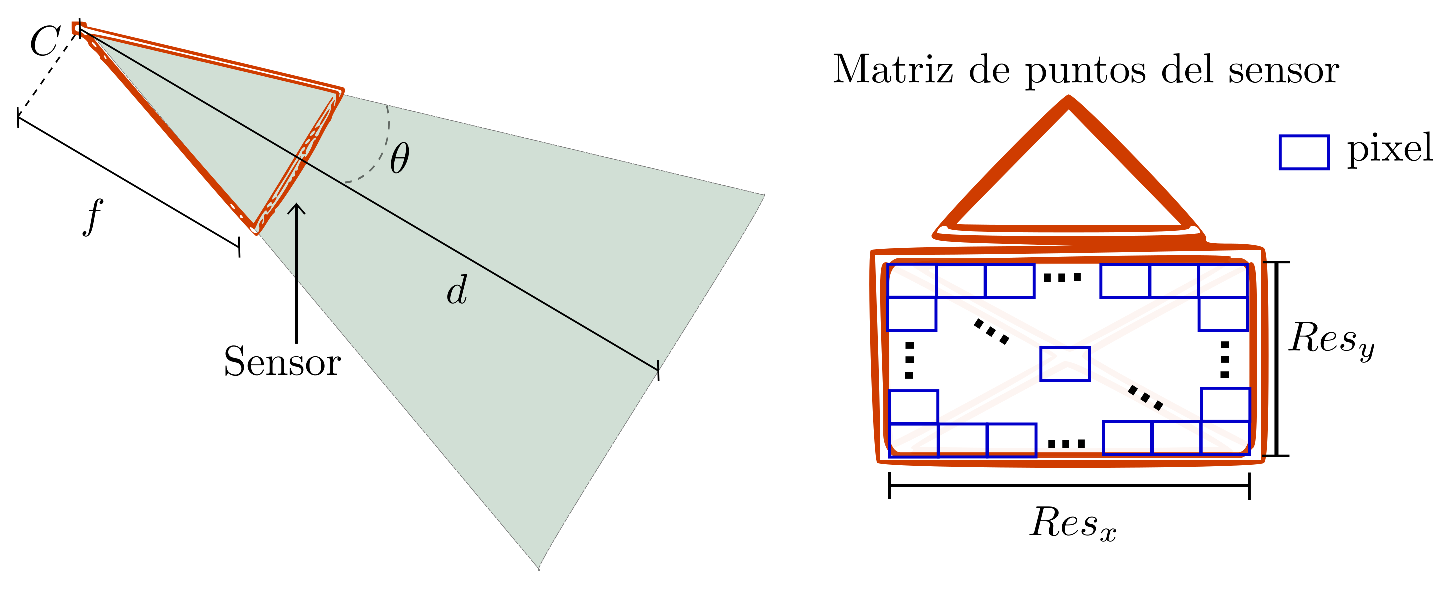
\includegraphics[scale=0.5]{img/Base_Datos/camara_resolucion.eps}}      
  \caption{Estimación del la resolución espacial.}
  \label{estimacion_resolucion}
\end{figure} 

Sean $x_s$ e $y_s$ magnitudes sobre el sensor de la cámara, horizontal y vertical respectivamente, y sea $X$ e $Y$ las magnitudes a una distancia $d$ del centro $C$ de la cámara que producen respectivamente las proyecciones de magnitud $x$ e $y$ sobre el sensor.
Se cumple la siguiente relación,
\begin{alignat*}{1}
X = \dfrac{d}{f}x_s&~, \quad \quad Y = \dfrac{d}{f}y_s
\end{alignat*}

Si el sensor\footnote{También referido como retina de la cámara.} tiene un largo $S_x$ y ancho $S_y$ y resolución de $R_x\times R_y$ píxeles, resulta que el largo de un píxel es $l_x = S_x/R_x $ y el ancho $l_y = S_y/ R_y$. 

A modo de ejemplo, se considera una cámara con las siguientes características $S_x = 0.032\;m$ y $S_y = 0.010\; m$, resolución de $1600\times600$ píxeles y una distancia focal de $32~mm$. Por lo tanto el error de un píxel se mapea sobre el sensor como $x = 0,032/1600\;m = 0.020\;mm$ a lo largo, e $y = 0.010/600\;m= 0.016\;mm$ a lo ancho. La Tabla \ref{table_resolucion} muestra como  errores de 1, 2 y 3 píxeles en el sensor se propagan sobre el espacio a una distancia $d$ del centro de la cámara.
\begin{table}[H]
\centering
\begin{tabular}{|c|l|l|l|l|l|}
\hline
\multirow{2}{*}{\begin{tabular}[c]{@{}c@{}}\textbf{número} \\\textbf{ de píxeles}\end{tabular}} & \multicolumn{5}{c|}{\textbf{d (metros)}} \\ \cline{2-6} 
                                                                              &\textbf{ 0,5}  &\textbf{ 1,0}  & \textbf{3,0}  & \textbf{5,0} & \textbf{10,0}\\ \hline
\textbf{1}                                                                             &  0,03    &  0,06    &   0,19   &  0,31   & 0,63      \\ \hline
\textbf{2}                                                                             &  0,06    &  0,12    &  0,38    &  0,62   &  1,26    \\ \hline
\textbf{3}                                                                            &   0,09   &  0,18    &  0,57    & 0,93    &  1.89    \\ \hline
\end{tabular}
\caption{Resolución espacial en centímetros como función de la distancia al centro de la cámara}
\label{table_resolucion}
\end{table}


\subsection{Marcadores}
A la hora de seleccionar el equipamiento se debe prestar especial atención y coordinar el tipo de marcador, la vestimenta del sujeto, el fondo del espacio de captura y el tipo de iluminación. Pues las características de estos elementos en conjunto pueden cambiar sensiblemente la performance del sistema que procesa computacionalmente la captura, sobre todo en sus primeras etapas tales como la detección de marcadores y la  calibración.
Si se quiere facilitar la tarea de detección automática de marcadores, estos deben ser fácilmente distinguibles del resto del entorno, y visibles la mayor cantidad de tiempo para las cámaras. Para ello se debe tener marcadores que generen un alto contraste con el resto de los elementos dentro de la captura de video. 
Su tamaño y forma también son importantes, por lo general se trabaja con marcadores esféricos, y un tamaño que dado cierto espacio de trabajo no condicione fuertemente la resolución necesaria de las cámaras. Una medida que se puede considerar aceptable con cámaras convencionales y movimientos a menos de 12 metros del centro de las cámaras, son marcadores de $3~cm$ de diámetro.  
Si el fondo del espacio de captura es negro, opaco, al igual que la vestimenta del sujeto a capturar, los marcadores pueden ser blancos, no pulidos de manera que su reflejo sea difuso, para no generar variación de tono sobre los mismos. 
Su disposición sobre el sujeto responde a los intereses de lo que se quiera observar, pero se debe tener presente que al ser una captura óptica, para que un marcador sea útil, debe estar visibles buena parte del tiempo en la secuencia.

\subsection{Iluminación}
La iluminación debería ser preferiblemente uniforme, para no generar sombras que modifiquen los tonos del espacio de captura. La luz natural es una buena alternativa, en espacios cerrados lo que habitualmente se utilizan son pantallas delante de los focos lumínicos para hacerlos más difusos, reduciendo así el riesgo de generar imágenes especulares en los objetos. La disposición de los focos depende de la forma del espacio de captura, pero por lo general rodean al mismo, cuidando que estos no sean capturados directamente por las cámaras, y generen falsos positivos en la detección de marcadores. Si bien esto último puede ser solucionado parcialmente en la etapa de  post-procesamiento efectuando convenientemente sustracción de fondo, es recomendable tratarlo en las primeras etapas, a nivel del sistema de captura. 

\subsection{Vestimenta}
Es preferible que la vestimenta del sujeto a relevar, consista en ropas finas y ajustadas para despreciar fluctuaciones de la posición de marcadores debido al movimiento de la ropa. Como se menciona anteriormente al igual que el fondo, la elección del color y material debe contrastar con los marcadores.

\subsection{Espacio de captura}

Ya se han mencionado algunas características cualitativas relacionadas con el espacio de captura, como ser que el fondo debe contrastar con los marcadores. Un caso interesante a tener en cuenta es el del túnel biométrico de la Universidad de Southampton mencionado en la Sección \ref{USlab}, donde para lograr dicho contraste utilizan patrones asimétricos con colores saturados para el fondo del espacio de captura, esto les permite agrupar dos etapas, logrando luego de un tratamiento sobre la secuencia, extraer el fondo del resto de la información y efectuar la calibración de las cámaras. De todas maneras si bien se mantienen relacionadas, las etapas mencionadas se manejan comúnmente por separado. Por lo que si se utilizan marcadores blancos, un fondo oscuro idealmente negro, y opaco es suficiente.\\

En cuanto a las dimensiones del espacio de captura, el mismo depende principalmente del tipo de movimiento a relevar y las características de las cámaras utilizadas. A continuación se analiza posibles configuraciones para dos caso, la marcha rectilínea y marcha libre, en el último caso se permite al sujeto movilizarse sobre un área circular.


\begin{figure}[ht!]
  \centering
  {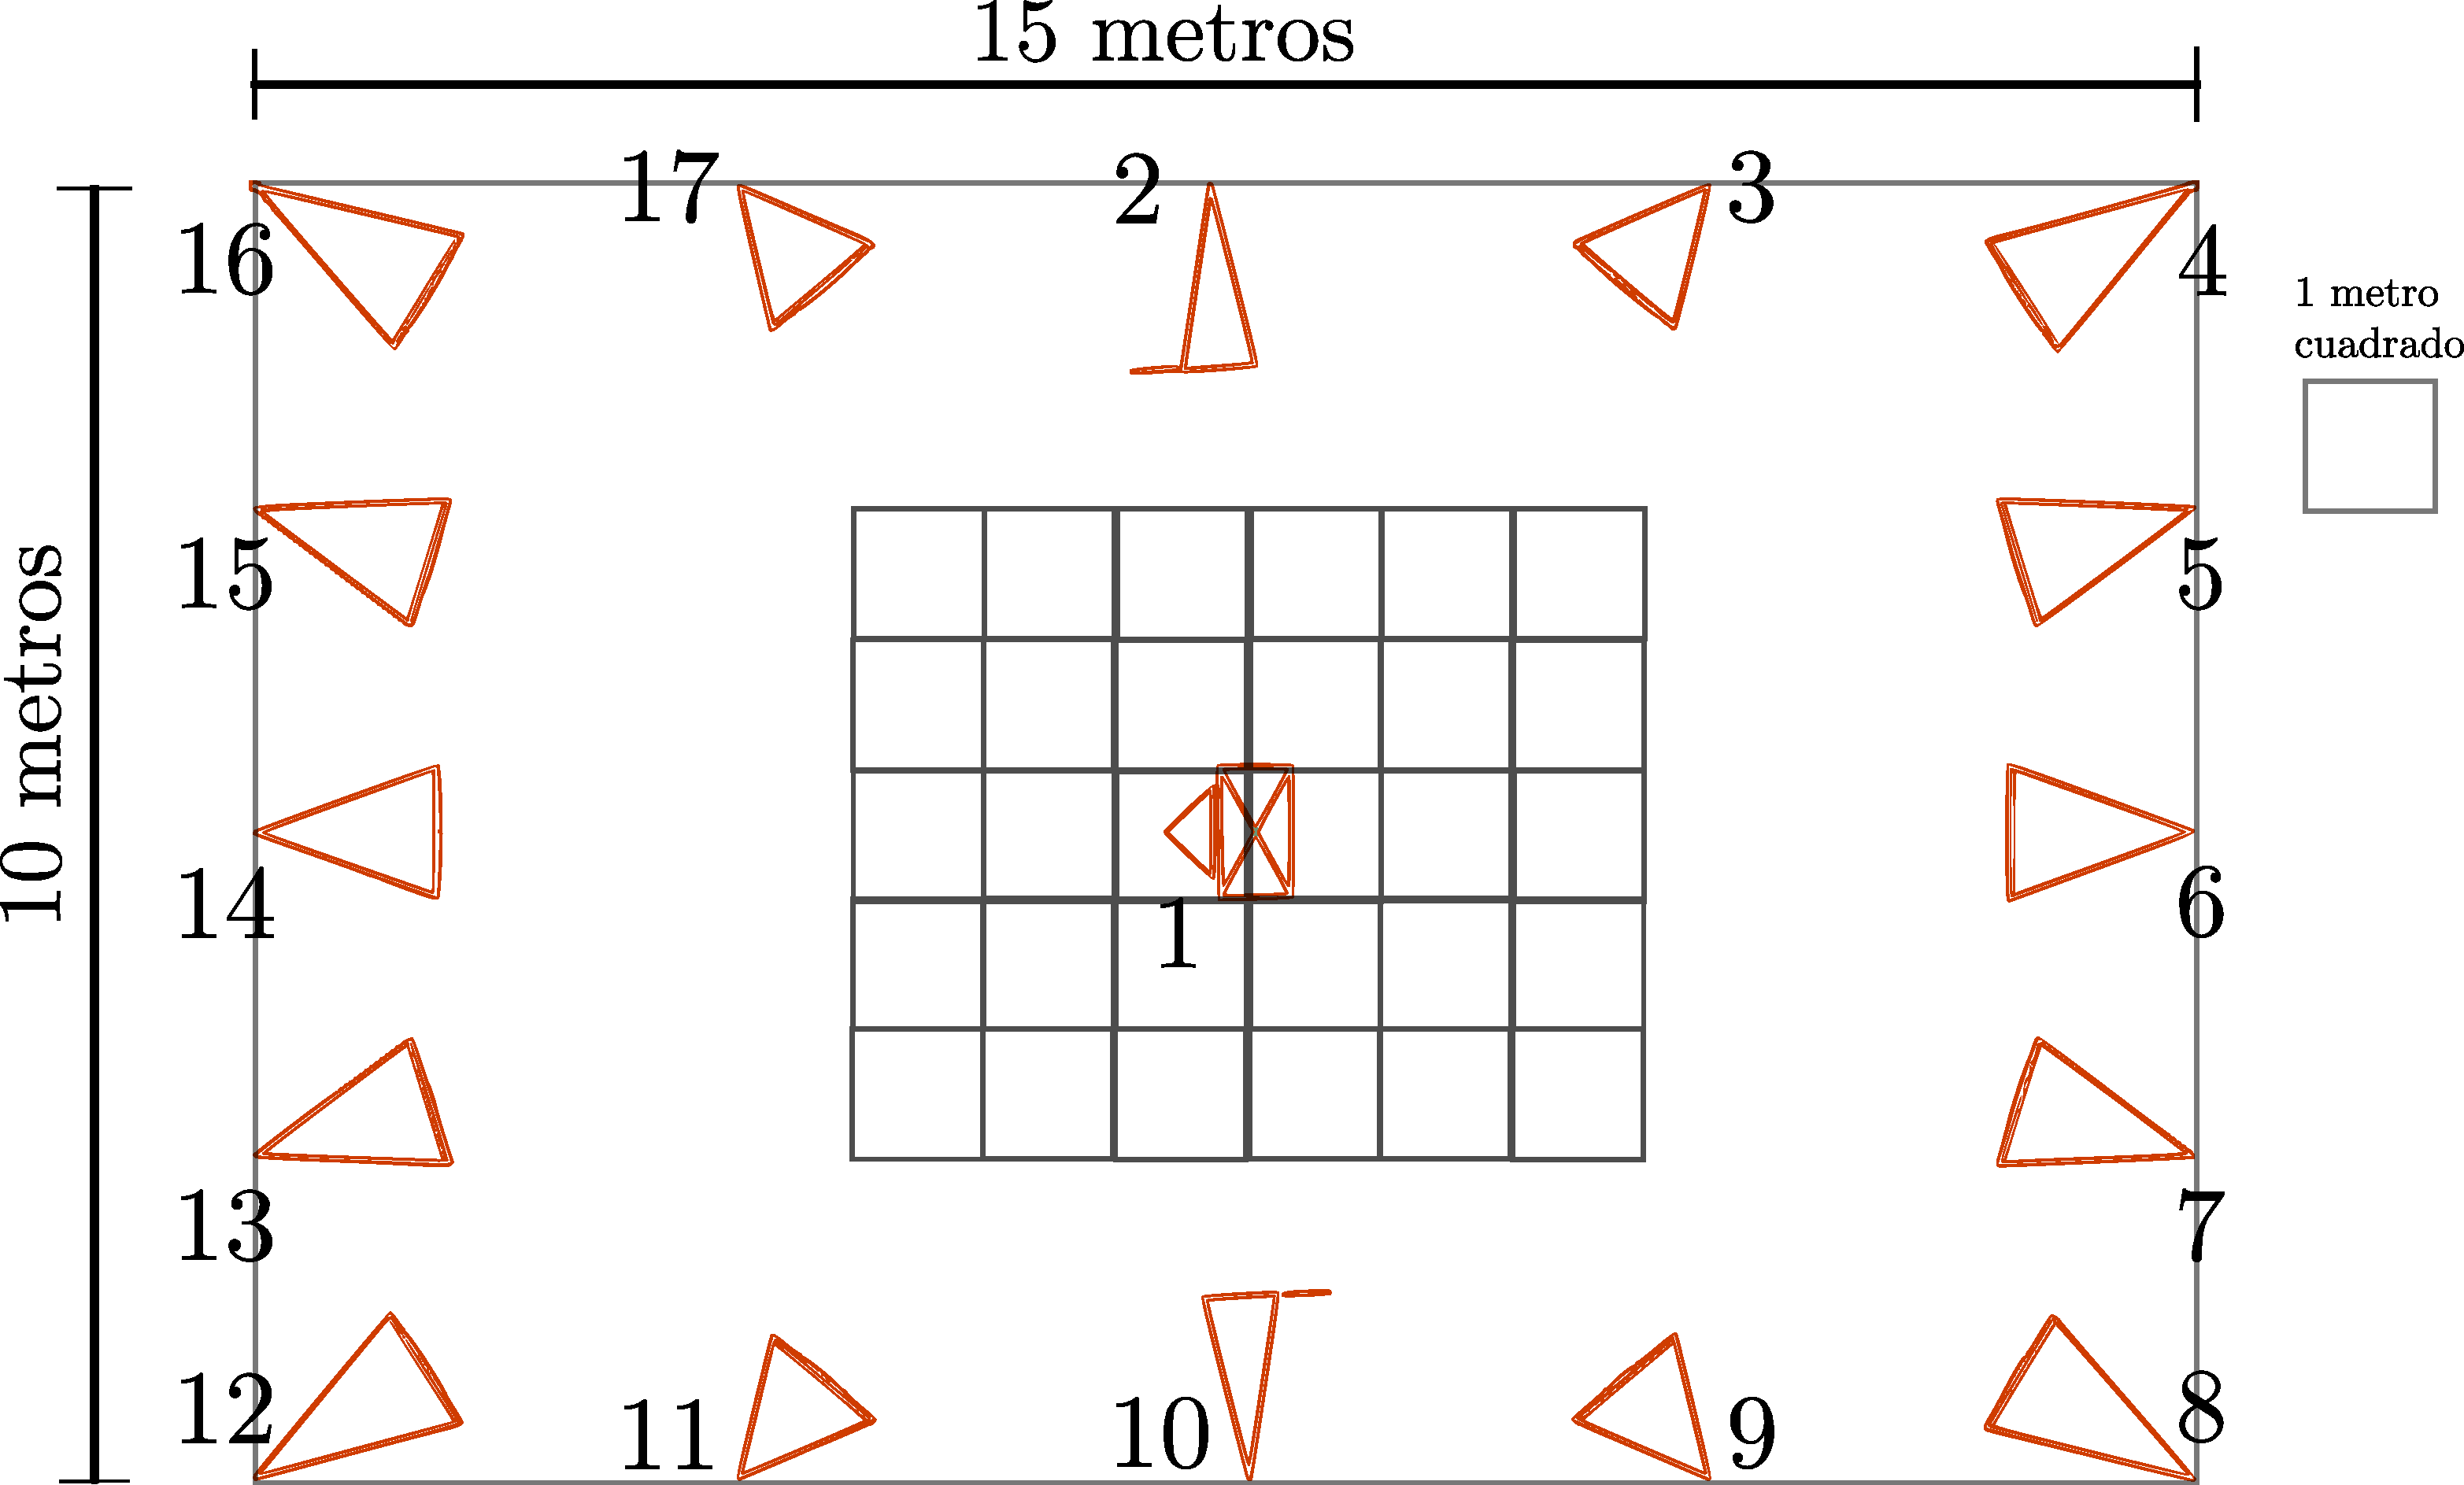
\includegraphics[scale=0.16]{img/Base_Datos/Laboratorio.pdf}}      
  \caption{Toma superior del Laboratorio.\\ Todas las cámaras se encuentran a $1\;m$ del suelo.}
  \label{img_Laboratorio}
\end{figure}  
 
 
\begin{figure}[ht!]
  \centering
  \hspace{-1cm}
   \subfloat[Espacio de captura para marcha rectilínea.]{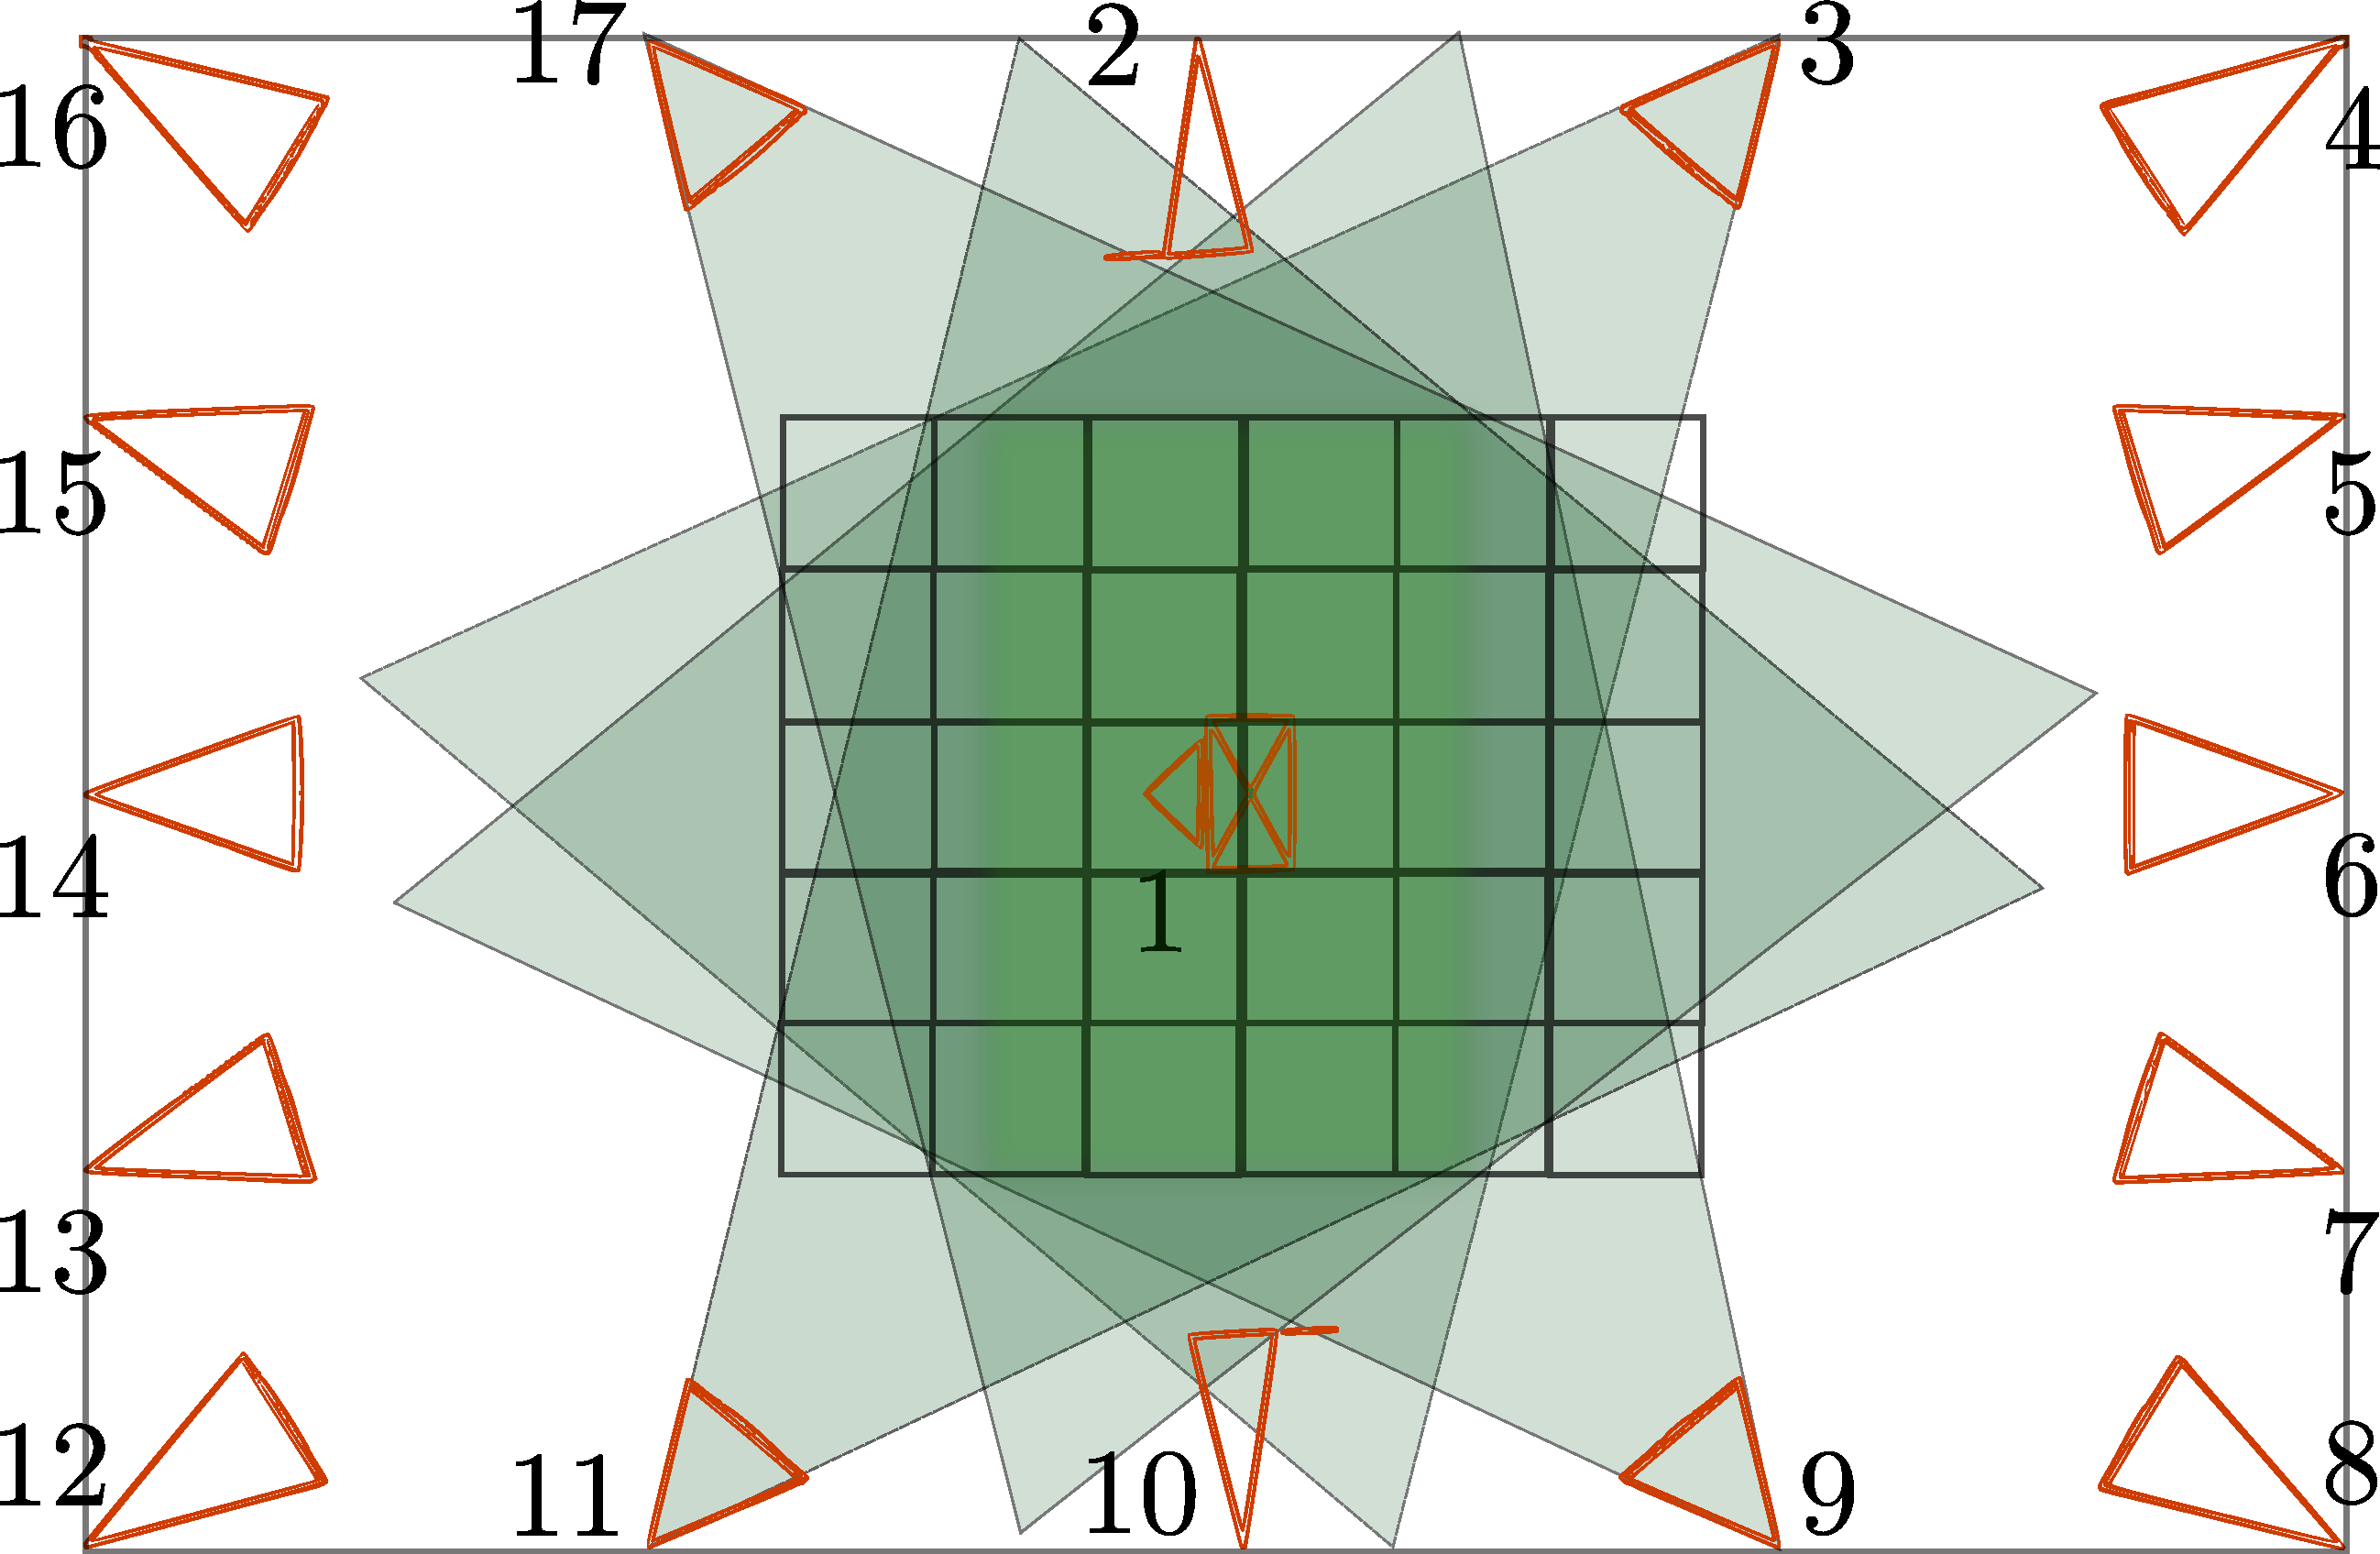
\includegraphics[scale=0.16]{img/Base_Datos/Lab_marcha1.pdf}\label{img_marcha1}}\hspace{0.3cm}
   \subfloat[Espacio de captura para marcha libre.] {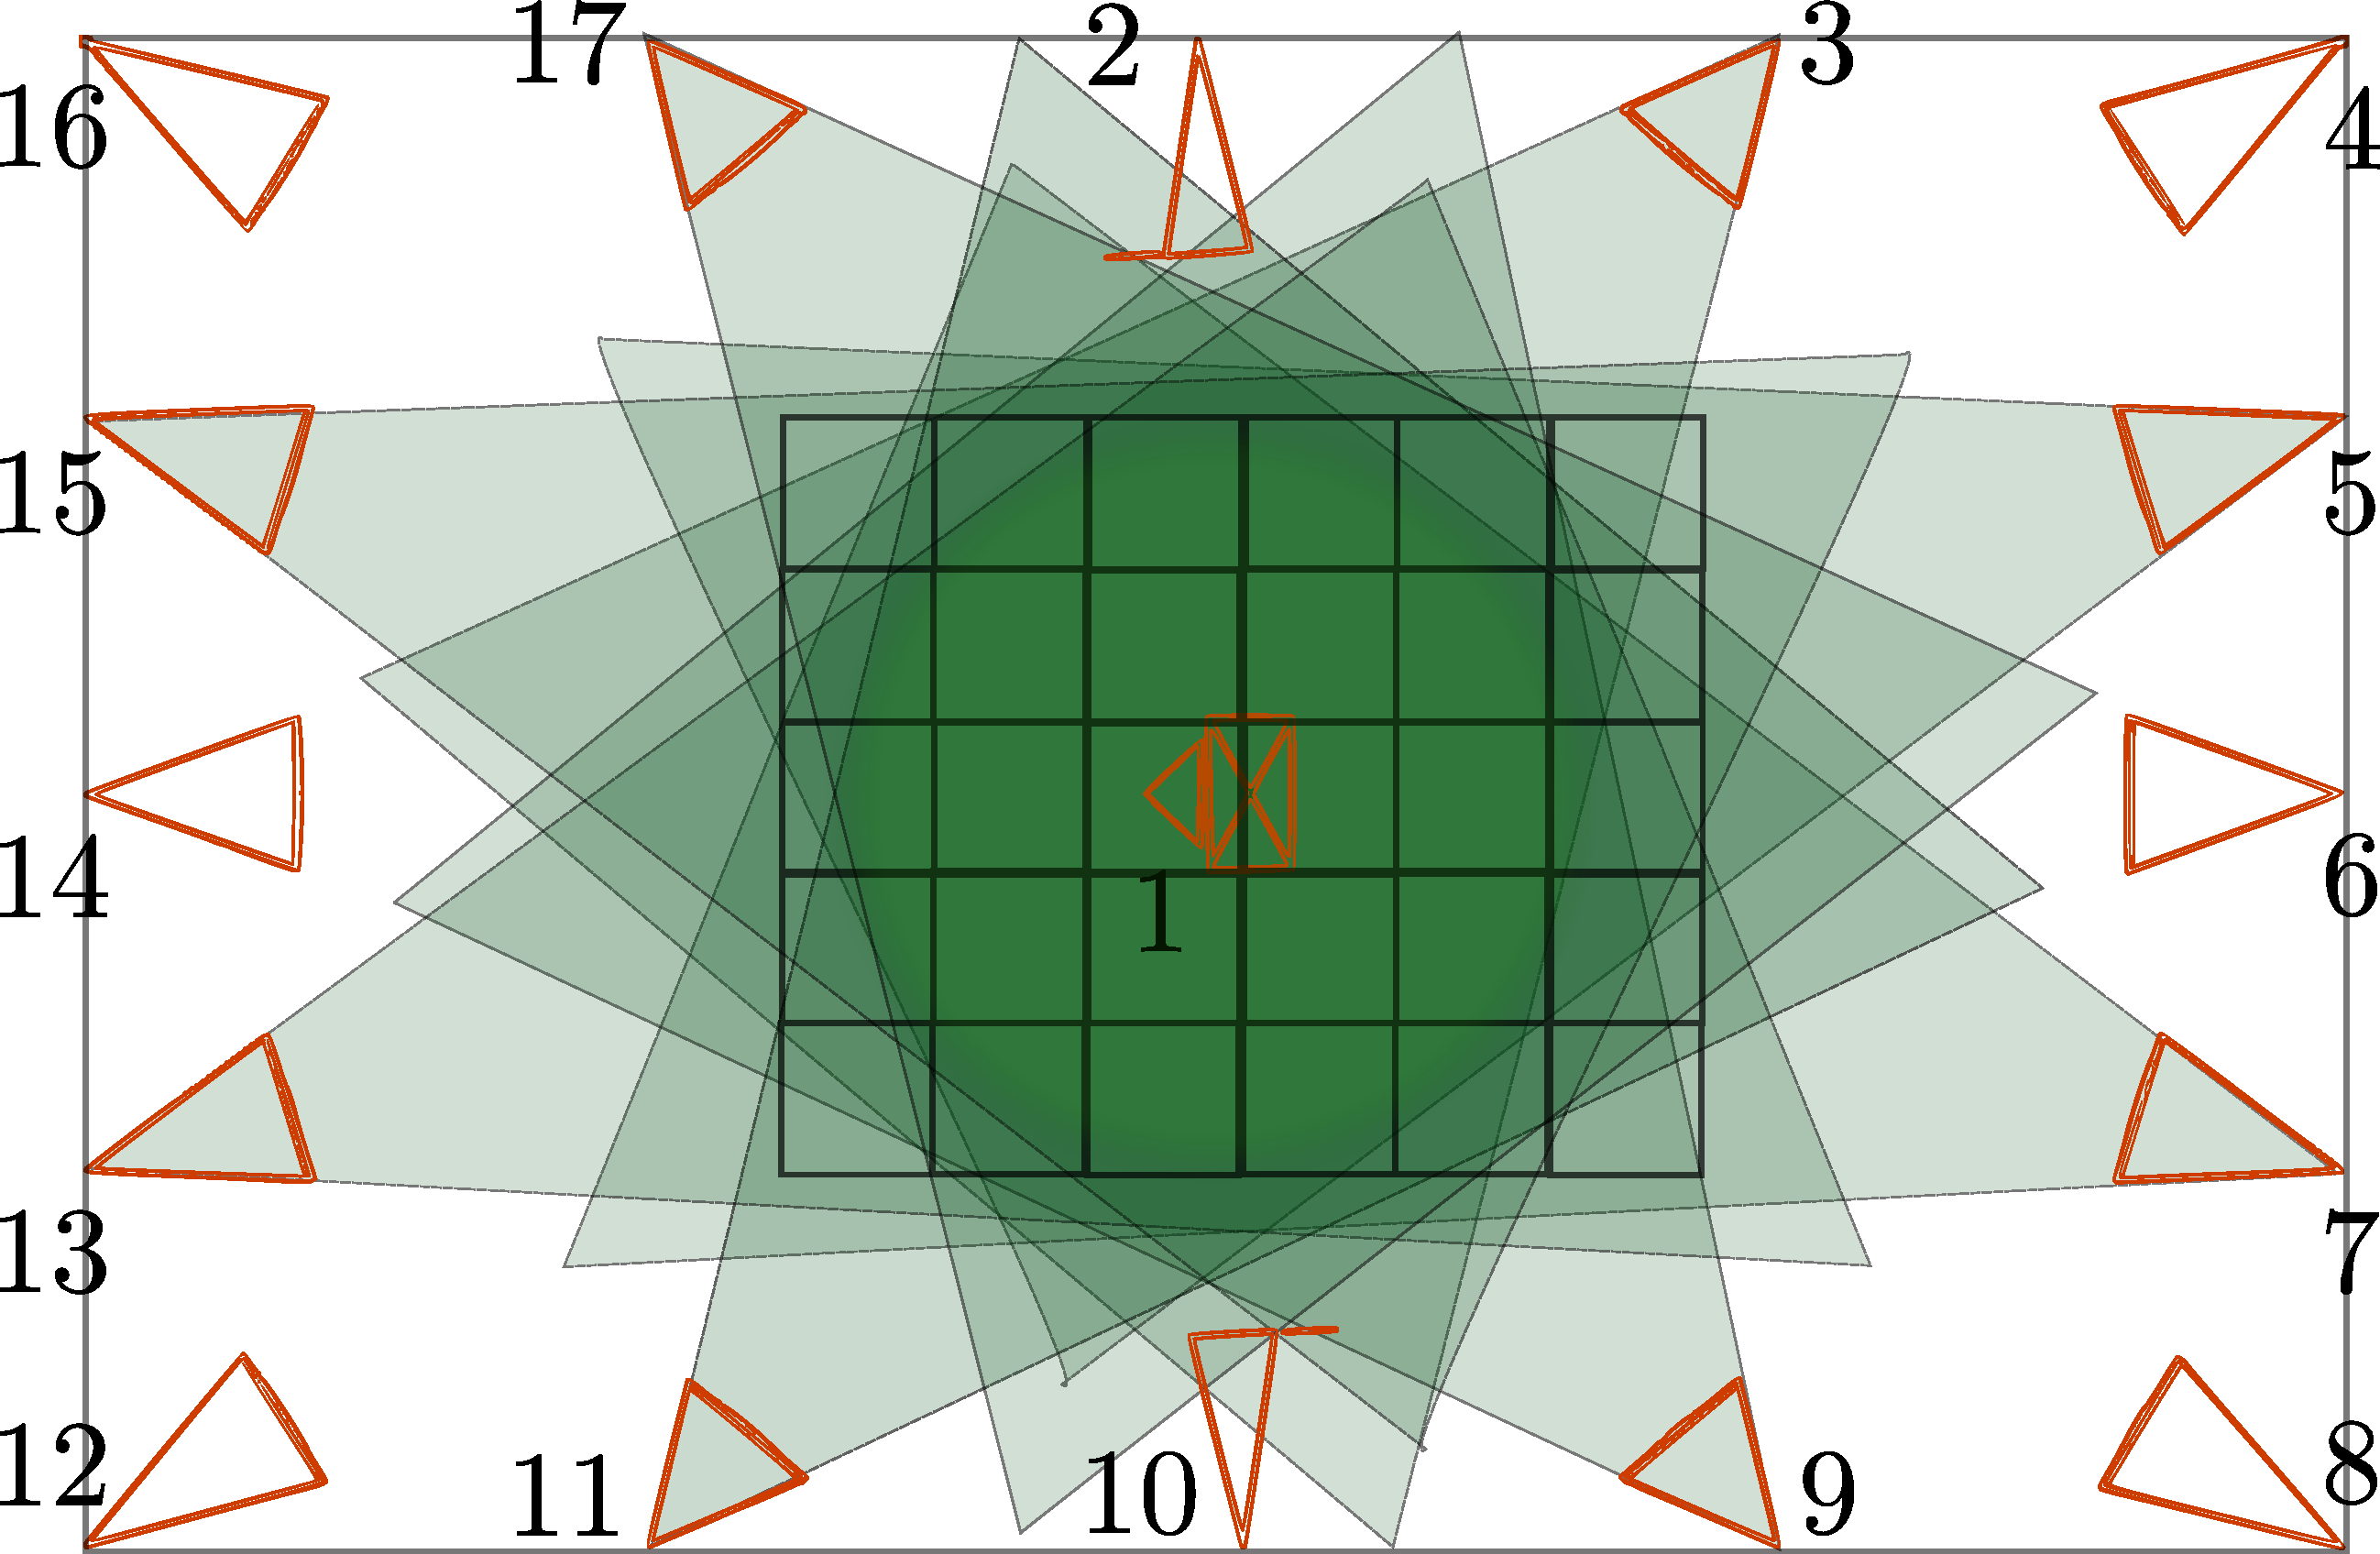
\includegraphics[scale=0.16]{img/Base_Datos/Lab_marcha2.pdf}\label{img_marcha2}}  \caption{Posibles espacios de captura.}
  \label{img_espacio_capura}
\end{figure} 
 
En el caso de la marcha rectilínea puede verse que en principio con tan solo cuatro cámaras dispuestas como en la Figura \ref{img_marcha1} se genera un espacio de captura útil de aproximadamente $3\;m\times5\; m$ en forma de pasarela. Si el sujeto restringe su movimiento sobre esta zona, dado que la misma se ubica dentro de la intersección de los campos visuales, será visto en su totalidad por todas las cámaras de manera simultánea. En el caso de marcha libre se disponen 8 cámaras intentando que el espacio de captura no tenga direcciones privilegiadas, con lo cual se genera una circunferencia, que en este caso es de aproximadamente $5\;m$ de diámetro. 


Siguiendo el proceso discutido anteriormente en la Sección \ref{parrafo_Camaras}, se puede estimar la resolución esperada en los datos obtenidos a partir de las secuencias de video, si se cuenta en principio con información de la resolución de las cámaras y su distancia focal. Consideremos nuevamente cámaras con resolución de $1600\times600$ píxeles y distancia focal de $f=32\;mm$, la mayor distancia sobre la cual una cámara debe tener cobertura en la pasarela de la Figura \ref{img_marcha1} es de $8 \;m$, mientras que en la Figura  \ref{img_marcha2}, caso de la marcha libre, es de $9\;m$ con lo cual un error de un píxel en una cámara produce una incertidumbre de aproximadamente poco más de medio centímetro en ambos casos a la hora de efectuar la reconstrucción con las secuencias de video obtenidas. 
Debe tenerse presente que estos son casos particulares, pero que permiten hacer una idea de las consideraciones a tener en cuenta para cumplir algunos de los requerimientos del sistema. 
Aumentar el número de cámaras permite una mayor cobertura de volumen, lo que significa una mayor visibilidad del conjunto de marcadores. A su vez una mejor visibilidad del conjunto de marcadores está correlacionado con disminuir la posibilidad de que información importante se pierda en las etapas de análisis de datos posteriores.


\subsection{Sincronización} 

Esto resulta esencial en las emisiones con conexiones en directo con varias cámaras, para garantizar que las imágenes de vídeo se mantienen estables incluso cuando se cambia de una cámara a otra.
Se debe contar con una fuente central que envíe una señal de sincronización a todas las videocámaras que participan en una grabación, de esta manera se indica a cada una de ellas cuando deberán comenzar a grabar. 
Esta señal de sincronización puede consistir en eventos sonoros o visuales que permitan sincronizar en etapas de post-procesamiento, pero lo más recomendable si se dispone de equipamiento adecuado es directamente enviar una señal a las cámaras vía hardware.
Si no se contara con una entrada de sincronización sería prácticamente imposible realizar una grabación con varias cámaras simultáneamente.



%
%
%\subsubsection{Conclusiones} 
%
%
%A la hora de configurar un laboratorio no solo hay que integrar las distintas variables, sino también cuidar que esta integración se gestione de manera compatible, de lo contrario se estaría desaprovechando el potencial de las secuencias generadas por el sistema de captura en cuanto al procesamiento posterior se trata. Dificultando la tarea de obtención de datos a partir de las secuencias de video.
%En esta sección se logra tratar algunos parámetros claves y se discute las relaciones que estos deben tener para generar capturas de movimiento con información óptica basada en marcadores de bueno calidad.
%
%
%A continuación se enumeran consideraciones de parámetros importantes para generar capturas en el caso de la marcha.
%
%Es deseable para una buena resolución temporal poseer cámaras que permitan capturar 30 cuadros por segundo, con tiempos de obturación de al menos $1/2000\, s$, esto último permite evitar efectos de distorsión debidos a falta de nitidez. La resolución espacial de los datos en el procesamiento condiciona la resolución de la cámara. Se concluye que trabajando a 10 metros con resolución $1600\times600$ se obtienen incertidumbres de píxel de casi $1 ~cm $. 
%
%
%El color de los  marcadores debe contrastar claramente con la vestimenta y el fondo del espacio de captura, se recomienda una forma esférica. En capturas con cámaras ubicadas a menos de 12 metros del movimiento a relevar, un tamaño aceptable para el marcadores es de $3\,cm$ de diámetro.
%
%La vestimenta debe ser ajustada, para despreciar fluctuaciones en la posición de los marcadores. Y preferiblemente de igual color que el fondo.  
%
%En cuanto a la iluminación, la misma debe ser uniforme, por ello si se utiliza iluminación artificial con focos puntuales es habitual colocar pantallas delante de los focos.
%
%El espacio de captura debe contrastar con los marcadores, y sus dimensiones varían según el tipo de marcha a relevar. En caso de marcha rectilínea sobre una plataforma de $3\,m \times 5 \,m$ se encuentra que 4 son el mínimo número de cámaras que permiten relevar el movimiento de manera satisfactoria. Mientras  que en el caso de la marcha libre sobre una plataforma circular de $5\,m$ de diámetro, se recomienda la utilización de 8 cámaras. Una posible disposición de las mismas se muestra en la Figura \ref{img_espacio_capura}.
%


\section{Datos experimentales} \label{seccion_Base_Datos_Sintetica}
\subsection{Motivación}

No se encontraron base de datos acorde a las necesidades de este proyecto. Como se menciona en la Sección \ref{seccion_revision_base_datos} varios son los motivos, pero básicamente se debe a que ninguna se diseñó para el análisis óptico  con marcadores y no ofrecen secuencias de video utilizables para estos fines. Por lo tanto se plantea la necesidad de construir una base de datos adecuada que permita desarrollar este sistema. Esto último no estaba contemplado inicialmente en los tiempos del proyecto, sin embargo dada la importancia que posee para el desarrollo del sistema se re-formula el cronograma y se ajustan los objetivos. 


Una característica importante en muchas de las bases relevadas es la manera con la que habitualmente se obtiene el ground truth a partir de sistemas de captura de movimiento (MoCap), tales como Vicon \cite{vicon} o Impulse \cite{vicon},
estos sistemas devuelven información muy precisa sobre la ubicación 3D de marcadores ubicados sobre el sujeto a estudiar. Este tipo de base de datos con capturas de movimiento, se utilizan ampliamente en el ámbito de la animación por computadora, pues se carga la información de la captura al modelo 3D de interés y este efectúa la acción esperada con un alto nivel de realismo. 


Dada la complejidad material y logística de implementar una base de datos, los tiempos necesarios para desarrollar las herramientas de análisis del proyecto y su necesidad de secuencias útiles, junto con el potencial de la información obtenida en el relevamiento de dicha base y sus usos en otros ámbitos, se decide generar una base de datos sintética con el material MoCap utilizado como ground truth. Trabajando en esta dirección se generan secuencias en un ambiente totalmente controlado, donde se conoce el ground truth, simplificando el testeo de algoritmos sobre diferentes etapas del procesamiento y permitiendo incrementar gradualmente las dificultades  en cada ensayo, por ejemplo efectuando variaciones en el número o posición de las cámaras. Estas características permiten a su vez generar \emph{benchmark's} de algoritmos, de gran importancia para futuros desarrollos del sistema. 


Continuando en esta dirección al día de hoy, se cuenta con herramientas de código libre para generar una base de datos sintética que sea robusta, completa y extensible. Particularmente se trabajo con la suite de animación 3D \textit{Blender} \footnote{ Blender Foundation \textcolor{blue}{\underline{\url{http://www.blender.org/}}}}, generando un laboratorio en dicho entorno virtual. Para obtener las secuencias de video, se asocia a un modelo  virtual 3D la información de movimiento de interés obtenida a partir de sistemas MoCap, para luego generar secuencias animadas, las cuales por último, se renderizan sobre un cierto número de cámaras para generar secuencias de video conteniendo múltiples vistas del modelo original. Estas secuencias son las que se utilizaron para el desarrollo del sistema y permitieron generar una base de datos sintética. 


\subsection{Formatos Mocap}\label{formatos_MoCap}
La captura de movimiento (Mocap), es una técnica de grabación del movimiento bastante popular en el cual se generan animaciones humanas o animales en ámbitos virtuales a partir de modelos reales. Este tipo de técnicas han sido utilizadas desde hace más de una década en el ámbito del entretenimiento, tales como el cine o los videojuegos e incluso en el ámbito deportivo y médico. 


Importante en la mayoría de las bases de datos relevadas, incluso aquellas de análisis óptico, ya que los sistemas comerciales que efectúan este tipo de capturas devuelven datos con un alto nivel de precisión, por lo que se utilizan como ground truth y se comparan con datos obtenidos a partir de otros sistemas. La primera desventaja de todas estas prestaciones es su alto costo, bastante privativo en muchos ámbitos.

En la actualidad el éxito de las capturas de movimiento ha dado lugar a una serie de casos de producción que pueden registrar y proporcionar datos de movimiento, sin embargo muchas de las empresas han desarrollado su propio formato de archivo. Esto significa que los formatos de archivo de los datos de captura de movimiento
están lejos de unificarse en un estándar, sin embargo la naturaleza ASCII de muchos de los formatos, hace que sea razonablemente fácil decodificar y entender la información por simple inspección de los datos.

\begin{table}[ht!]
\caption{Formatos de archivo Mocap.}
\label{tabla_Mocap_extensions}
\begin{minipage}{\textwidth}
\centering
\begin{tabular}{|l|l|}
\hline
\textbf{Formatos Mocap} & \multicolumn{1}{c|}{\textbf{Compañía}}                                              \\ \hline
ASF \& AMC              & Acclaim \footnote{\textcolor{blue}{\underline{\url{http://www.darwin3d.com/gamedev/acclaim.zip }}}. Accedido 30-11-14}                                                                            \\ \hline
BVA \& BVH              & BioVision \footnote{\textcolor{blue}{\underline{\url{http://www.biovision.com/bvh.html }}}. Accedido 30-11-14}                                                                          \\ \hline
BRD                     & LambSoft Magnetic Format \footnote{\textcolor{blue}{\underline{\url{http://www.dcs.shef.ac.uk/~mikem/fileformats/brd.html}}}. Accedido 30-11-14}                                                           \\ \hline
C3D                     & \begin{tabular}[c]{@{}l@{}}Biomechanics, Animation and\\ Gait Analysis \footnote{\textcolor{blue}{\underline{\url{http://www.c3d.org/c3d_format.htm }}}. Accedido 30-11-14}\end{tabular} \\ \hline
CSM                     & \begin{tabular}[c]{@{}l@{}}3D Studio Max, \\ Character Studio\footnote{\textcolor{blue}{\underline{\url{http://www.dcs.shef.ac.uk/~mikem/fileformats/csm.html}}}. Accedido 30-11-14}\end{tabular}          \\ \hline
GTR, HTR \& TRC         & Motion Analysis \footnote{\textcolor{blue}{\underline{\url{http://research.cs.wisc.edu/graphics/Courses/cs-838-1999/Jeff/MoCapTOC.html}}}. Accedido 30-11-14}                                                                    \\ \hline
\end{tabular}
\end{minipage}
\end{table}
La aplicación que se realice condiciona cual de los formatos de la Tabla \ref{tabla_Mocap_extensions} es más conveniente. 
La mayoría de los formatos mostrados son soportados por \textit{Blender}, sin embargo dado que en este caso el interés es la manipulación y fácil interpretación de la información, el formato elegido para manipular las capturas de movimientos es el BVH, por ser posiblemente el más compacto, conciso y ampliamente utilizado. De todas maneras se cuenta con funciones en \textit{Matlab} para llevar la información de movimiento contenida en estos archivos a varios de los formatos descriptos en la Tabla \ref{tabla_Mocap_extensions}, así como también directamente a una matriz con las coordenadas 3D de cada marcador a lo largo del tiempo.

\paragraph{BVH (BioVision Hierarchical data).}

El formato BVH proviene del formato BVA de BioVision con la notable adición de una estructura de datos jerárquica que representa los huesos\footnote{Entidad básica en la representación del esqueleto. Cada hueso representa el segmento más pequeña dentro del movimiento sujeto a cambios de traslación y rotación. } del esqueleto\footnote{Entidad global que representa el movimiento. Un esqueleto está formado por huesos.}. Se compone de dos partes, la primera sección detalla la jerarquía y la pose inicial del esqueleto y la segunda sección el movimiento del mismo, describiendo la información temporal del esqueleto cuadro a cuadro.
 
 
\begin{figure}[ht!]
  \centering 
  \hspace{0.5cm}  
   \subfloat[Esqueleto]{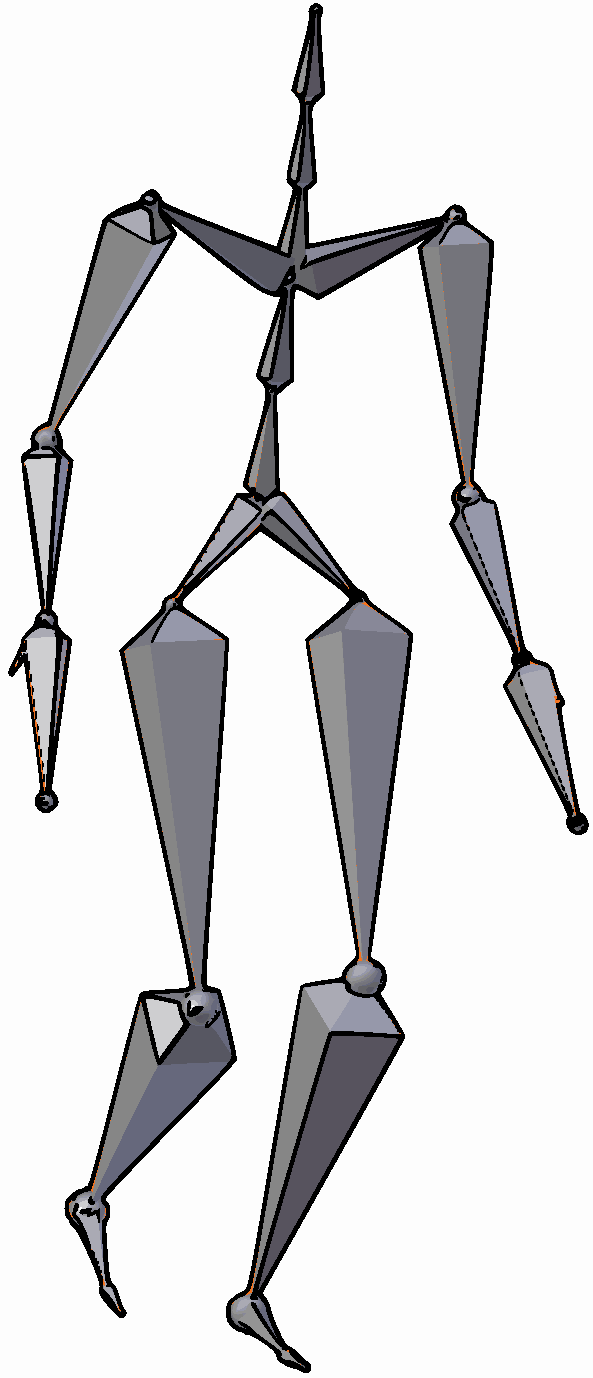
\includegraphics[scale=0.25]{img/Base_Datos/Estructura_esqueleto1.pdf}\label{img_Esqueleto_1}}\hspace{2.5cm}  
   \subfloat[Estructura jerárquica]{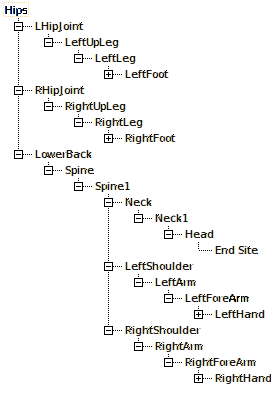
\includegraphics[scale=0.36]{img/Base_Datos/Estructura_bvh}\label{img_estructura_bvh}}\hspace{0.2cm}   
   \subfloat[Sección de jerarquía]{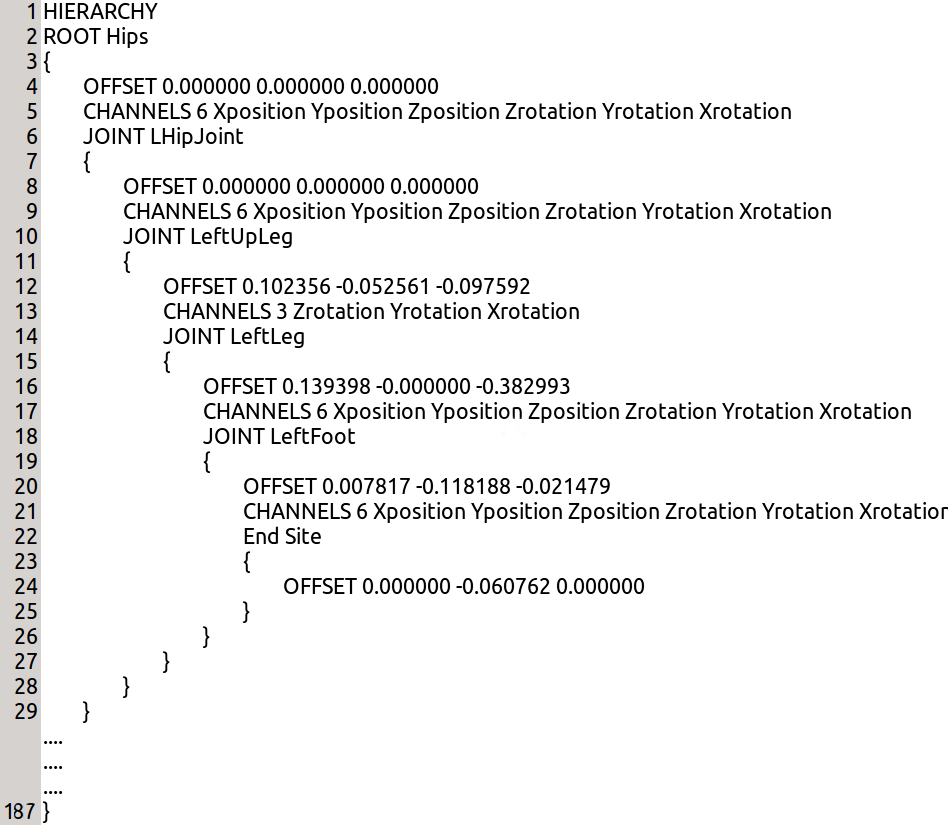
\includegraphics[scale=0.2]{img/Base_Datos/BVH_Encabezado.png}\label{img_BVH_Encabezado}}\hspace{0.01cm}   
   \subfloat[Sección de movimiento]{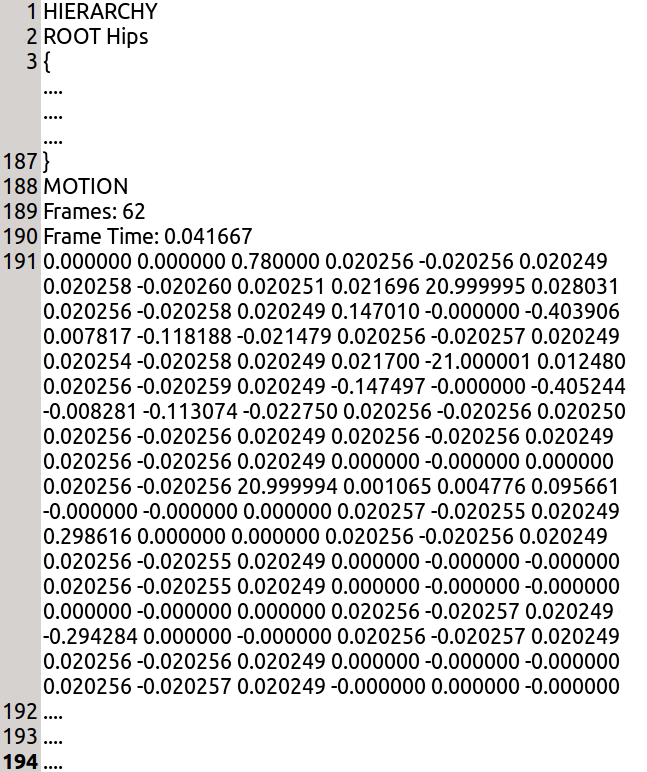
\includegraphics[scale=0.2]{img/Base_Datos/BVH_Motion.png}\label{img_BVH_Motion}}  
   \caption{Información contenida en archivos BVH.}  
\end{figure}   

La sección jerárquica del archivo empieza con las dos primeras líneas conteniendo las palabras HIERARCHY y ROOT respectivamente, seguidas del nombre del hueso que es la raíz de la estructura jerárquica y a continuación la estructura restante del esqueleto definida de manera recursiva conteniendo la información del origen de cada hueso y el orden en que las variables del hueso se modifican en la segunda sección. La sección de movimiento empieza con la palabra clave MOTION, contiene la cantidad de cuadros en la secuencia, el tiempo entre cuadros y la  información completa de la posición de cada hueso del esqueleto en cada cuadro de la secuencia. Por más detalles del formato consultar el artículo de M. Meredith y S.Maddock \cite{meredith2001motion}.  

Si bien en principio cualquier fuente de archivos BVH con capturas de movimiento es válida, se decide trabajar en este proyecto con las fuentes BVH de la base de datos \textit{MotionBuilder-friendly version} ofrecidas por \textit{cgspeed} \cite{cgspeed}, 
%\footnote{\textcolor{blue}{\underline{\url{https://sites.google.com/a/cgspeed.com/cgspeed/motion-capture}}}. Accedido 4-12-14},
 que provienen de las capturas de Carnegie Mellon University Motion Capture Database \cite{CMU}.
 %\footnote{\textcolor{blue}{\underline{\url{http://mocap.cs.cmu.edu/}}}. Accedido 30-11-14}. 
 Como se menciona anteriormente en la Sección \ref{CMU}, CMU dispone de un gran número de capturas de movimiento de acceso público, varias utilidades de software que permiten llevar a otros formatos y es utilizado ampliamente en el ámbito de la animación por computadora.




\subsection{Laboratorio Virtual} %SECCIÓN EN CONSTRUCCIÓN\\
En esta sección se describe de que manera se puede utilizar \textit{Blender} y Python para generar secuencias de video para una base de datos sintética.

% % % % % % % % % % % % % % % % % % % % % % % % % % % % % %
% % % % % % % % % % % % % % % % % % % % % % % % % % % % % %
%Los parámetros de las distintas componentes así como los detalles de procesos enumerados en esta sección se encuentran en el apéndice (COLOCAR AQUÍ LA REFERENCIA PARA EL APÉNDICE).
% % % % % % % % % % % % % % % % % % % % % % % % % %
% % % % % % % % % % % % % % % % % % % % % % % % % % % %DESCOMENTAR AL HACER APÉNDICE




\textit{Blender} es una suite de animación 3D gratuita y de código abierto, la misma cuenta con las herramientas necesarias para trabajar en todas las etapas de desarrollo de un proyecto de animación 3D. Por otro lado posee una interfaz de programación de aplicaciones muy flexible y potente que permite extender su funcionalidad a través de programas en lenguaje Python. Estas cualidades son muy útiles para generar una base de datos por lo que se decidió desarrollar la misma utilizando las herramienta de esta aplicación.

Se ha generado un espacio de trabajo controlado, conteniendo entre otras cosas un cierto número de cámaras, iluminación, color de fondo determinado y un modelo con marcadores sobre el cual cargar la captura de movimiento de interés. También se han implementado programas en Python para facilitar múltiples tareas:

\begin{itemize}
\item  Ayudar en  el ajuste de las capturas provenientes de archivos BVH al esqueleto del modelo virtual.
\item	Generar las secuencias de video a partir de archivos .blend  con el modelo virtual desarrollando el movimiento de interés.
\item	Exportar la información de calibración de las cámaras en un archivo .m para usar la misma desde \textit{Matlab}.
\end{itemize}


\begin{figure}[ht!]
  %\centering 
  \hspace{-1.0cm}
   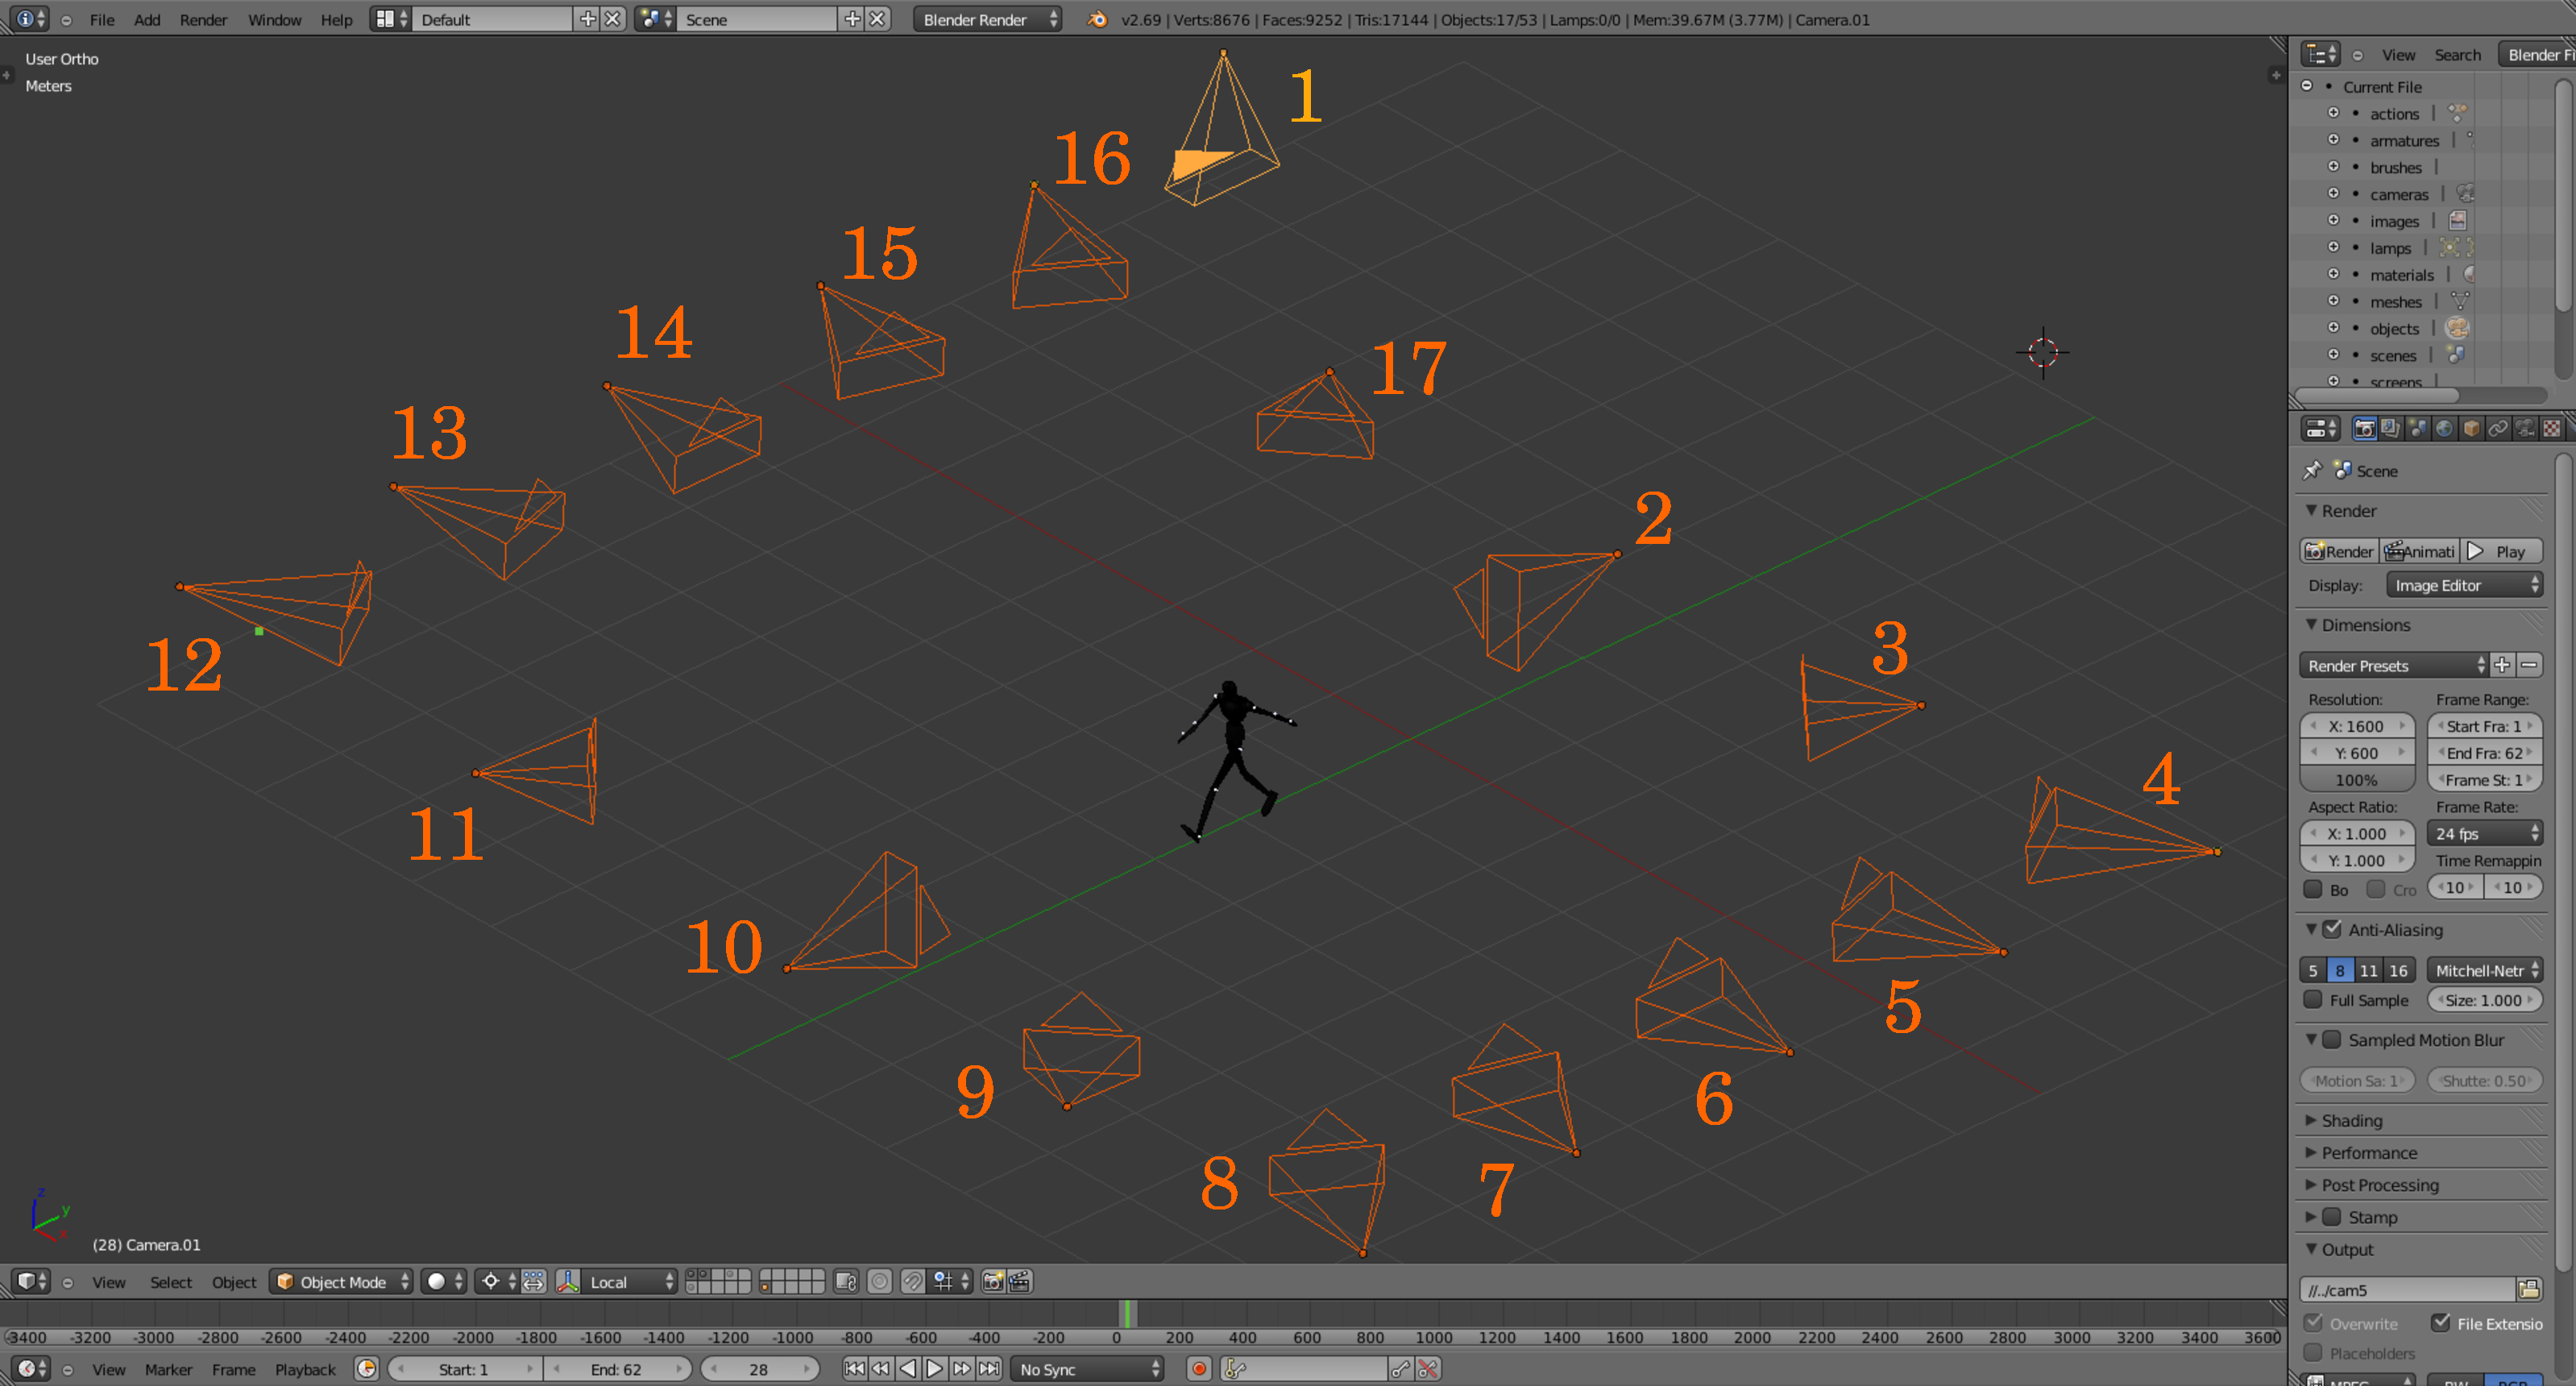
\includegraphics[scale=0.28]{img/Base_Datos/Entorno_Blender.pdf}
   \caption{Entorno de trabajo en \textit{Blender}.}
  \label{img_Entorno_Blender}
\end{figure}   


\subsubsection*{Disposición del laboratorio}
El laboratorio generado posee 17 cámaras dispuestas en un ambiente rectangular de $10\times15\;m $ como se muestran en las Figuras \ref{img_Laboratorio} y \ref{img_Entorno_Blender}. La configuración de las mismas permite probar diferentes combinaciones de captura a la hora de generar secuencias. Se diseñaron las cámaras para que sus parámetros fuesen similares a cámaras convencionales
 encontradas en el mercado y utilizadas en las bases de datos relevadas. 
 % % % % % % % % % % % % % % % % % % % % % % % % % % % % % % % %5
 % % % % % % % % % % % % % % % % % % % % % % % % % % % % % % % % %
% Las posiciones y valores característicos de las cámaras pueden verse en detalle en el apéndice  
% (PONER AQUÍ LA REFERENCIA AL APÉNDICE DONDE SE MUESTRA LA SALIDA DE INFOCAMBLENDER). 
% % % % % % % % % % % % % % % % % % % % % % % % % % % % % %
% % % % % % % % % % % % % % % % % % % % % % % % % % % % % % % % %DESCOMENTAR AL HACER APÉNDICE
Para iluminar el laboratorio se dispusieron $8$ focos puntuales de luz omnidireccional sobres los límites del mismo, rodeando la escena y a un nivel de 3 metros de altura. De esta manera se garantiza que ninguno de los focos sea tomado directamente por las cámaras y los marcadores se iluminan correctamente.
 

\subsubsection*{Modelo virtual}  
El modelo virtual utilizado se basa en un maniquí de madera convencional, la elección del mismo responde a la facilidad con la que se puede ajustar el mismo a una posición particular, siendo cada miembro fácilmente correlacionado con un hueso específico, sin perder las particularidades propia de un sujeto real. Cabe destacar que la relevancia del modelo en las capturas es simular las oclusiones de marcadores debida a los miembros del sujeto en una captura real.  

Para la elección del material aplicado al modelo virtual, se toman en cuenta las consideraciones planteadas en la Sección \ref{seccion_Caracteristicas_Laboratorio}, dado que los marcadores que se van a utilizar son de color difuso blanco, se decide aplicar sobre el modelo un material difuso negro con especularidad baja, de manera que no se generen brillos indeseados debido a la iluminación en el momento de la captura. De esta manera la configuración recomendada es utilizar un fondo también oscuro.

\subsubsection*{Esqueleto}
En cuanto a el esqueleto con la información de movimiento, el mismo se obtuvo de la base de datos \textit{MotionBuilder-friendly versión} (de aquí en más MotionBuilder) ofrecidas por \textit{cgspeed} \cite{cgspeed}, 
%\footnote{\textcolor{blue}{\underline{\url{https://sites.google.com/a/cgspeed.com/cgspeed/motion-capture}}}. Accedido 4-12-14},
 donde se cuenta con las fuentes BVH que provienen de las capturas de movimiento de CMU (Sección \ref{CMU}). Si bien\textit{ cgspeed} ofrece otras bases más nuevas, donde la jerarquía del esqueleto en los archivos BVH a sido reducida con el fin de facilitar el ajuste a modelos virtuales, se ha trabajado con la base original antes mencionada. Aparentemente el procesamiento aplicado para producir las nuevas bases, introdujo ruido sobre algunos cuadros en las secuencias originales, esto se ha constatado al importar en \textit{Blender} dichas secuencias.
      
 Con el fin de normalizar las secuencias BVH provenientes de MotionBuilder se ha utilizado la herramienta de edición de archivos BVH \textit{bvhacker} \cite{bvhacker}.
 %\footnote{bvhacker: The free bvh file editing tool. \textcolor{blue}{\underline{\url{ http://davedub.co.uk/bvhacker/}}}. Accedido 5-12-14}.
 La misma permite centrar las secuencias sobre un mismo punto en el primer cuadro removiendo los offset globales.
 Una vez gestionado lo anterior se importa en \textit{Blender} la secuencia BVH y se procede a generar los marcadores en las articulaciones del esqueleto, dado que se tiene la posición exacta del origen de cada hueso en el esqueleto y la articulación es la unión entre dos huesos consecutivos, se puede obtener la posición exacta de los marcadores a partir de la secuencia BVH.
 La generación de los marcadores y el enlazado del esqueleto al modelo se realiza a través de un código python, \texttt{acoplar\_modelo.py}, realizado para tal fin. El mismo genera marcadores esféricos de material difuso blanco levemente poroso, con $2,8 \;cm$ de diámetro y baja especularidad, centrados en las articulaciones definidas previamente en una lista, como se muestra en la Figura \ref{img_esqueleto_marcador} y luego enlaza cada miembro del modelo a su correspondiente hueso. De está manera para finalizar la creación del modelo con marcadores solo resta que el usuario realice ajuste mínimos de tamaño y posición sobre el modelo. Es importante resaltar que los marcadores se ubican sobre puntos del esqueleto de los cuales se conoce la posición 3D en cada cuadro y que el modelo es necesario debido a que el esqueleto no se puede renderizar. 
 
 \begin{figure}[ht!]
   
   \hspace{-1.0cm}
   \subfloat[Creación de marcadores]{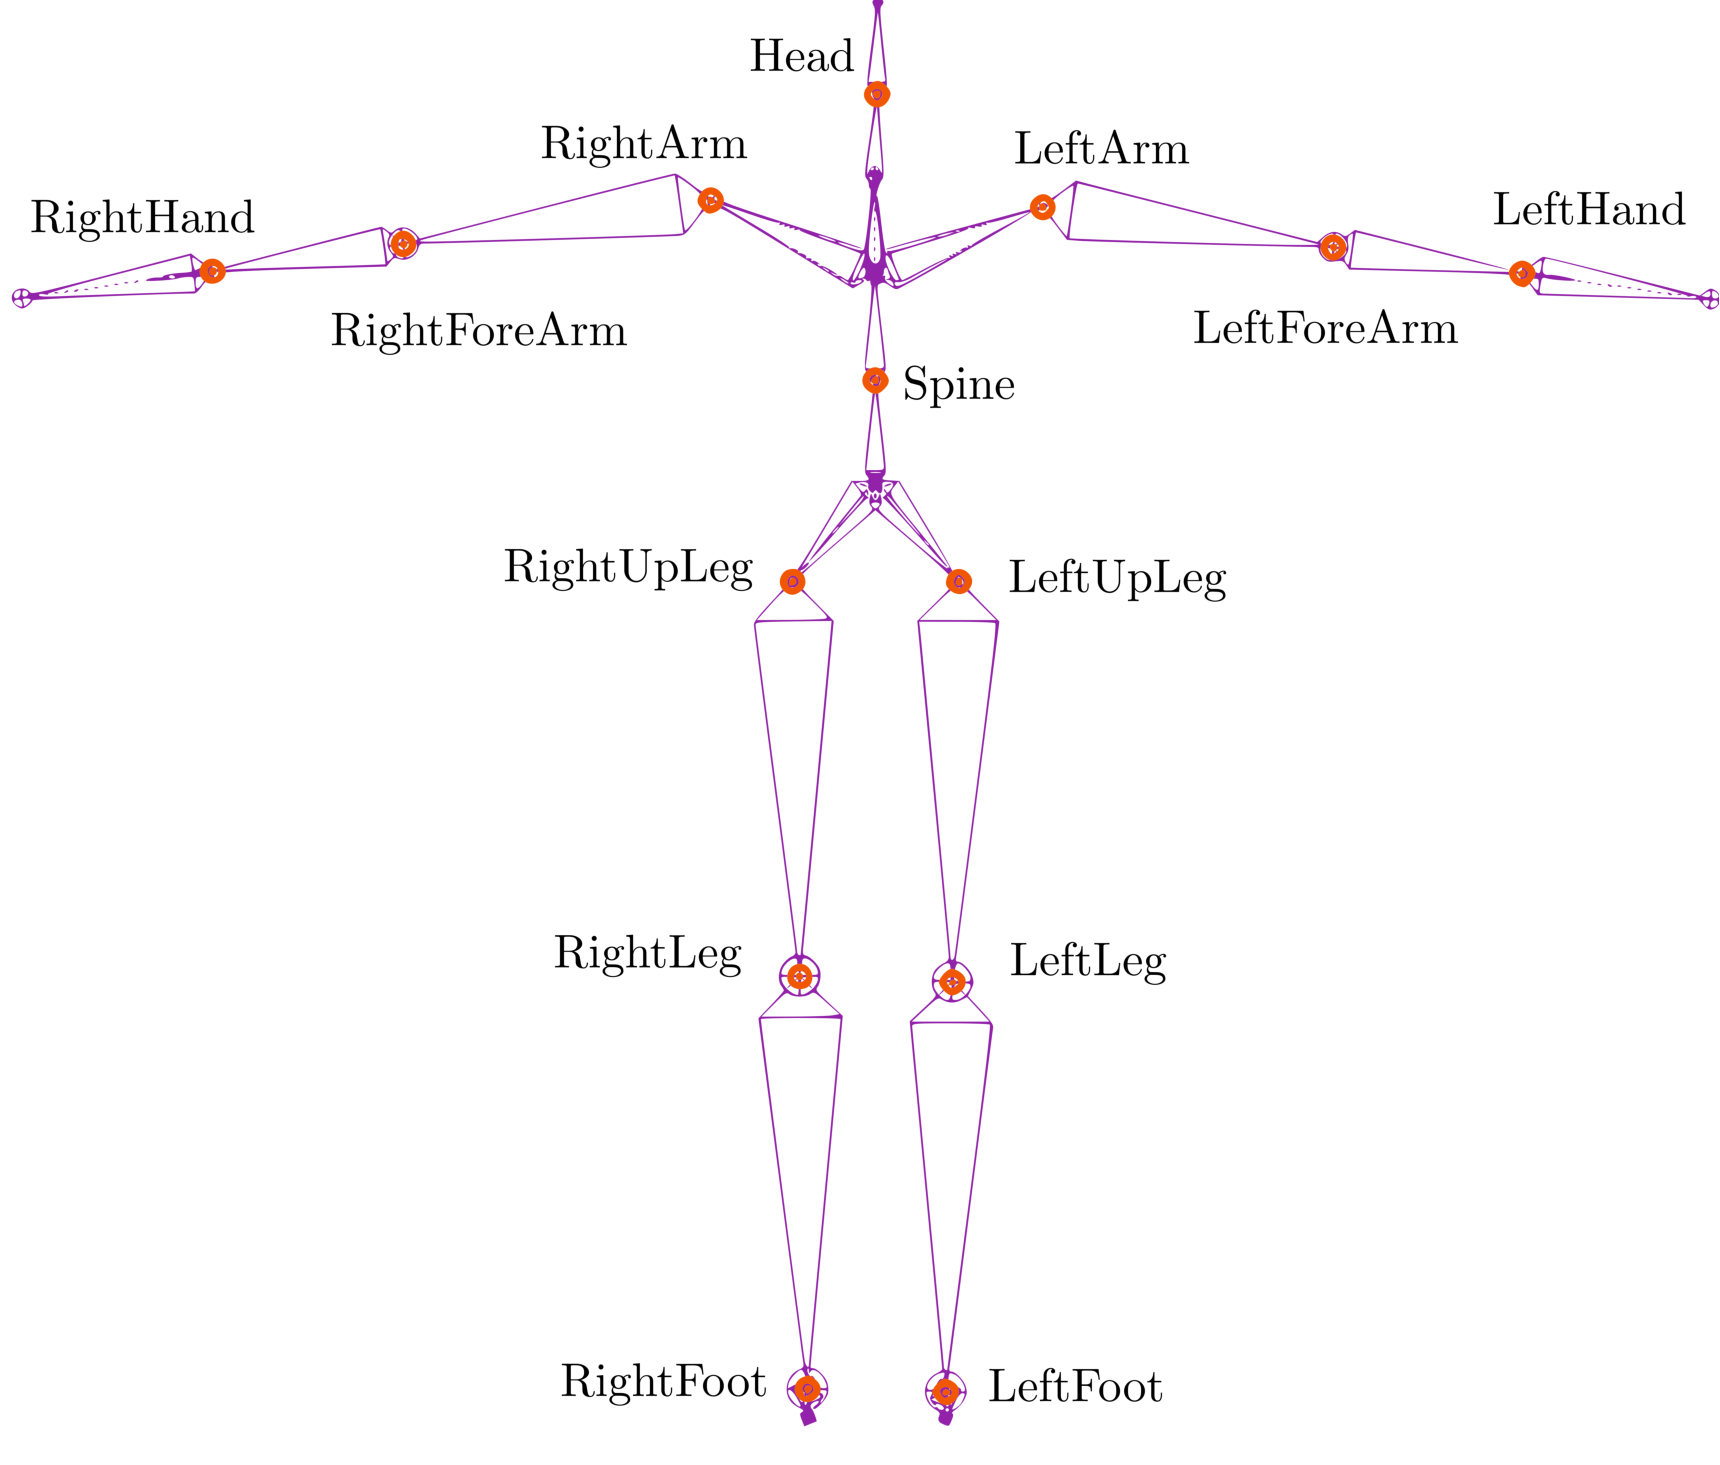
\includegraphics[scale=0.23]{img/Base_Datos/Esqueleto_Marcador.pdf}\label{img_esqueleto_marcador}} \hspace{0.6cm}
   \subfloat[Ajuste de modelo]{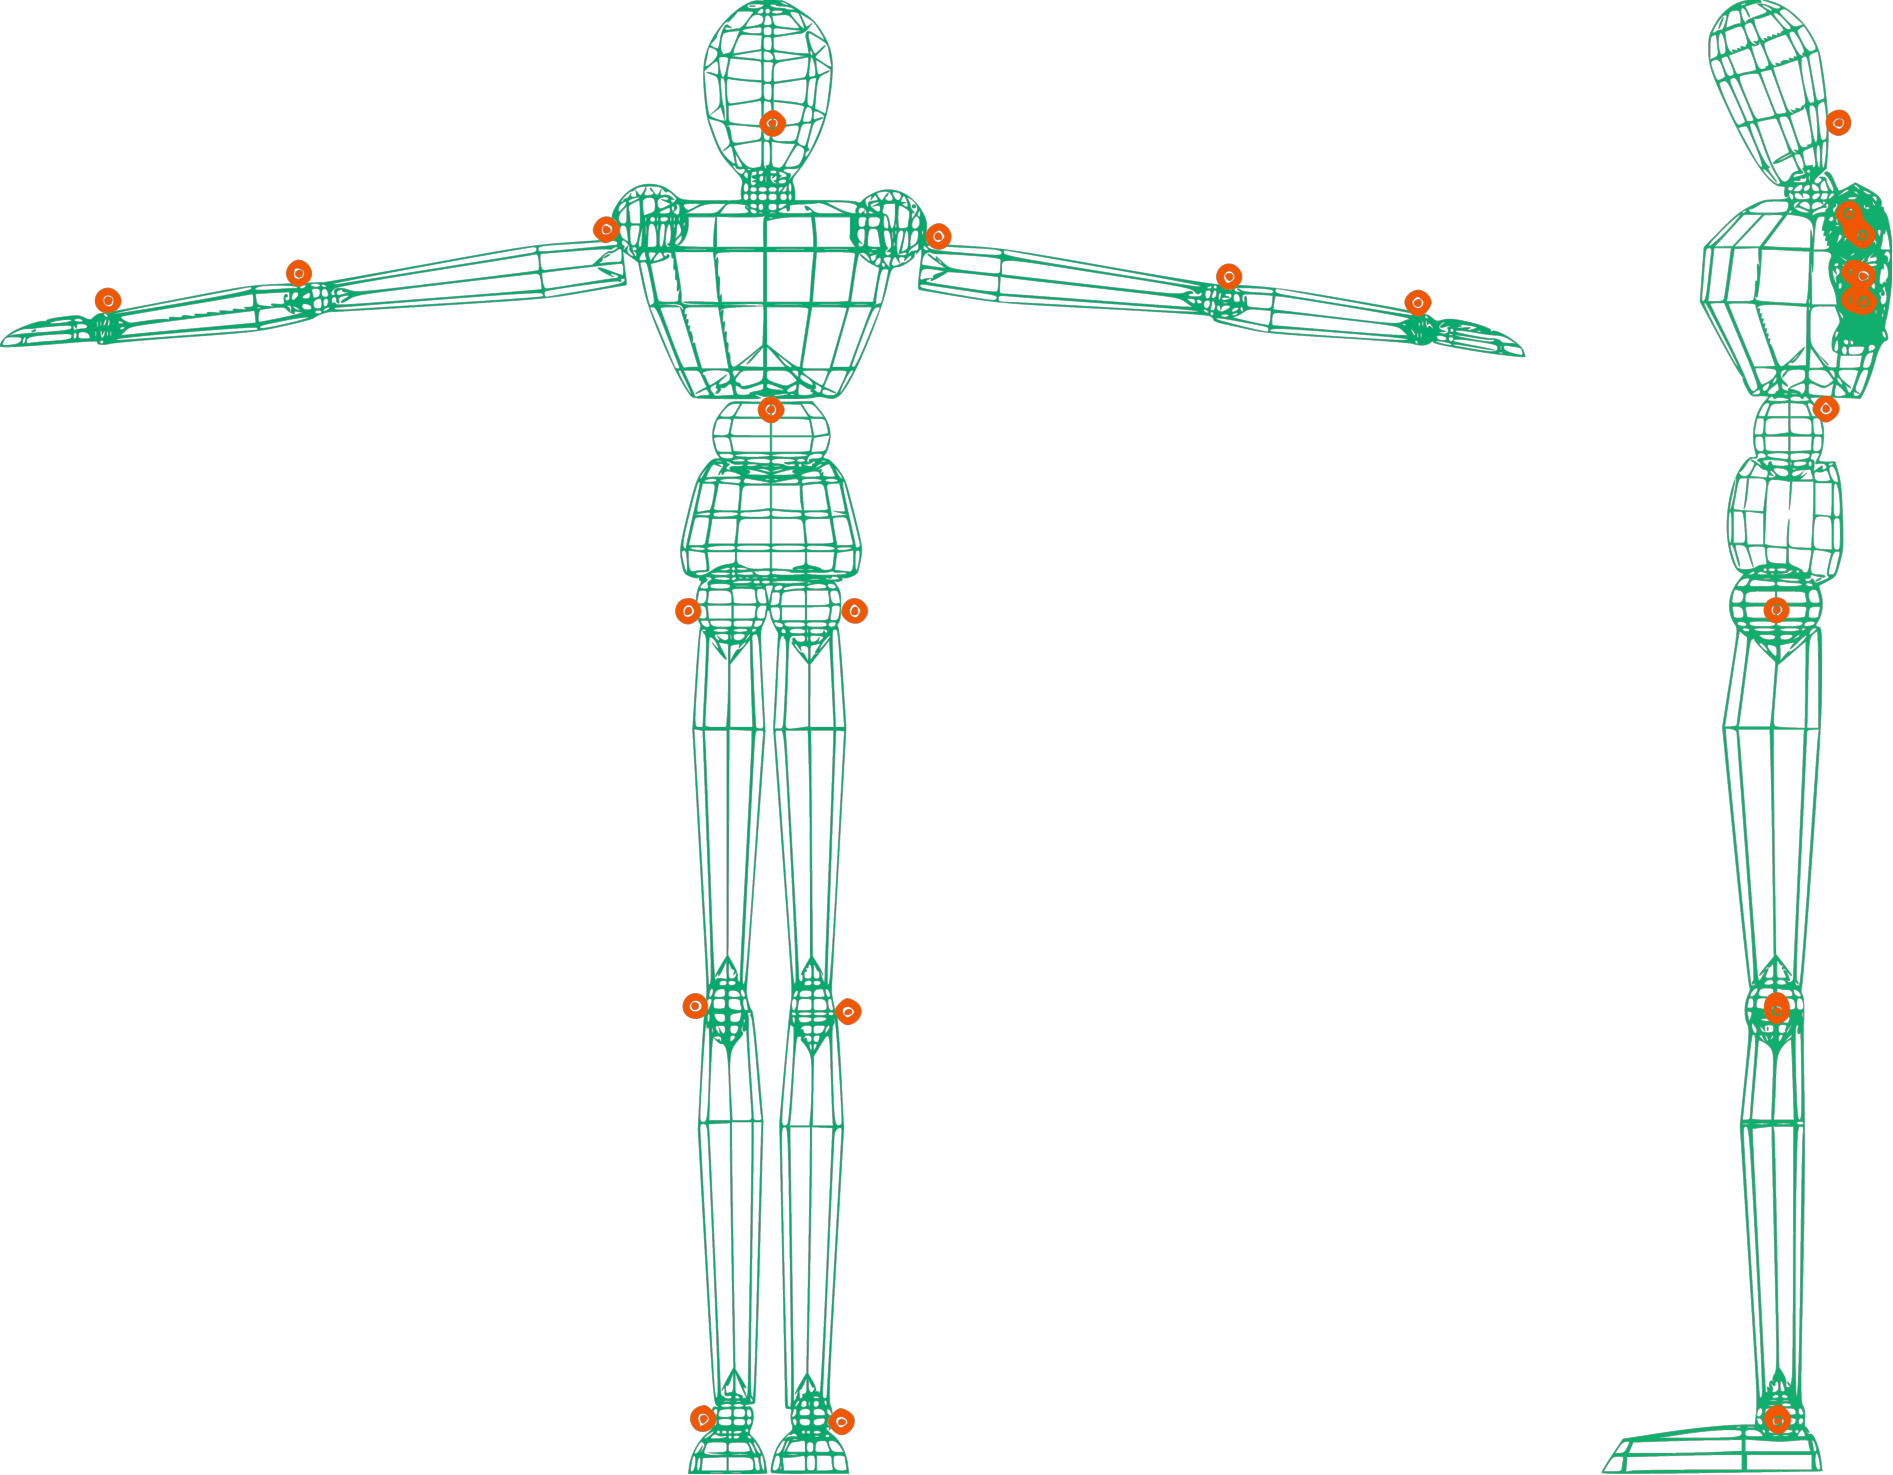
\includegraphics[scale=0.23]{img/Base_Datos/Modelo_Marcador.pdf}\label{img_modelo_marcador}}
   \caption{Generación de marcadores sobre el modelo virtual.}   
 \end{figure}  
 
Una ves finalizado el proceso, Figura \ref{img_modelo_marcador},  el modelo puede realizar el movimiento contenido en la secuencia BVH y solo resta renderizar. 

\subsubsection*{Renderizado} 

Ya se dispone de la secuencia de movimiento en el entorno virtual de \textit{Blender}, lo que resta es renderizar dicha secuencia sobre las cámaras del laboratorio. Para ello se implementó un código en python, \texttt{render.py},  que automatiza todo el proceso, dispone los videos obtenidos en cada render con nombres y ubicaciones predefinidas en la base de datos y genera un código \textit{Matlab} con la información ground truth de cada cámara. 


 \begin{figure}[ht!]
   \hspace{-1cm}
   \subfloat[Importación de secuencia BVH y generación de marcadores]{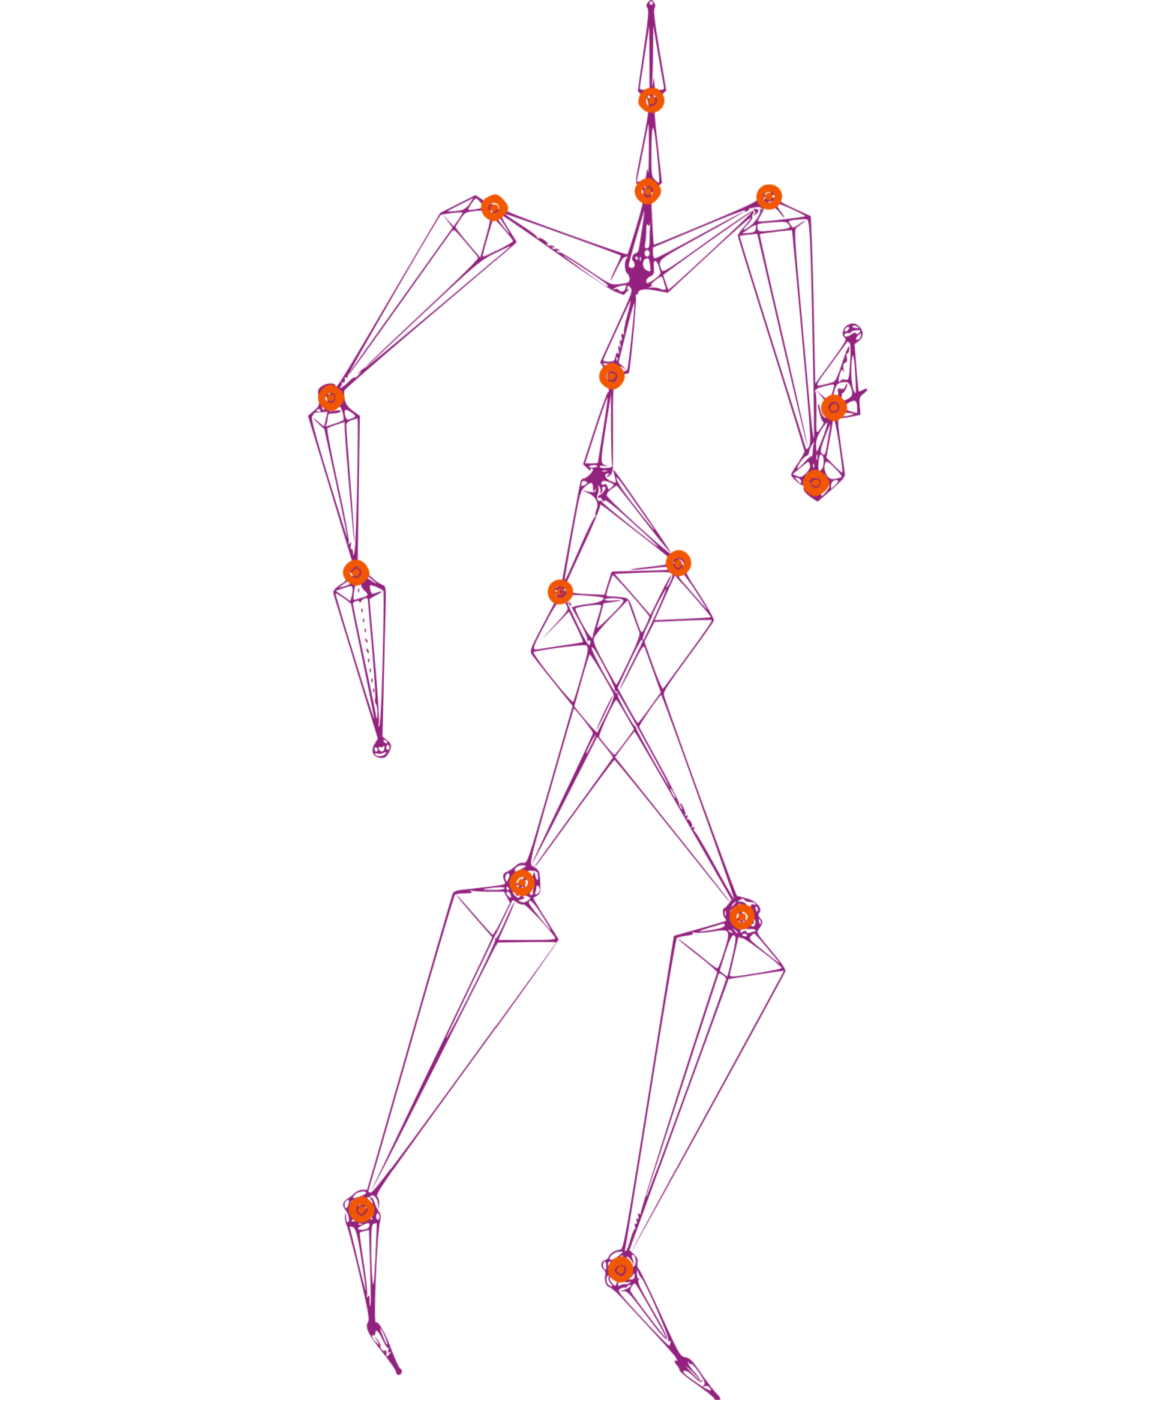
\includegraphics[scale=0.25]{img/Base_Datos/Esqueleto_Render.pdf}} \hspace{0.2cm}
   \subfloat[Modelo enlazado al esqueleto]{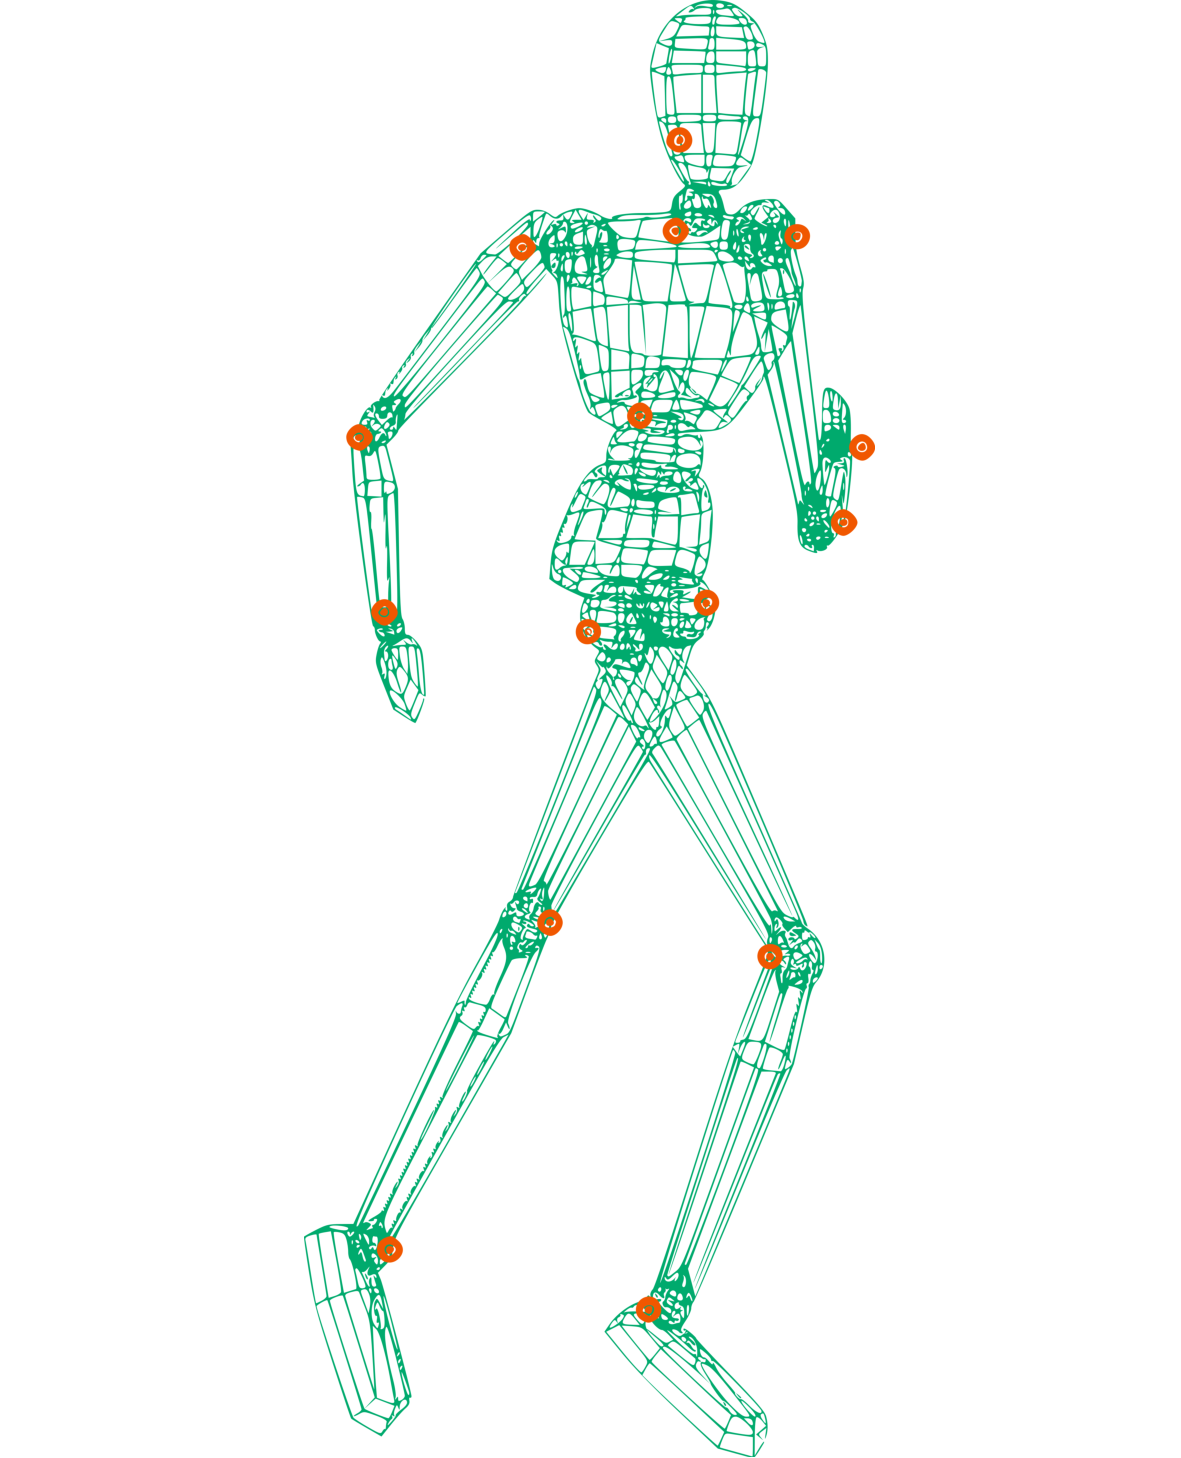
\includegraphics[scale=0.25]{img/Base_Datos/Modelo_Render.pdf}}
   \hspace{0.2cm}
   \subfloat[Imagen renderizada]{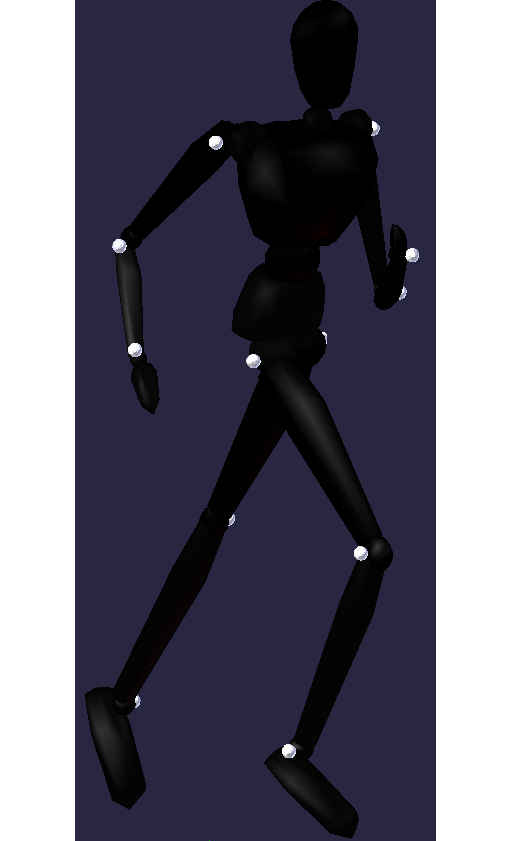
\includegraphics[scale=0.205]{img/Base_Datos/Modelo_Render2.png}}
   \caption{Creación de secuencias en \textit{Blender}.}   
 \end{figure} 


 
\subsubsection*{Ground truth} 

Para contar con el ground truth final de la secuencia animada se debe exportar desde \textit{Blender} la información del esqueleto en un BVH, cuidando que se mantenga la misma escala de tiempos que en el momento del renderizado. De esta manera se tienen sincronizados los videos y el ground truth 3D.

\subsubsection*{Mocap Tools}

Existe una herramienta en \textit{Blender} que permite manipular y copiar la información de movimiento entre dos esqueletos, denominada \textit{Mocap Tools}. La misma no viene activada por defecto y se debe habilitar desde el menú de preferencias. Para la creación de secuencias utilizando esta herramienta, se debe tener un esqueleto ya enlazado al modelo virtual con marcadores, luego se importa la secuencia BVH de interés que a su vez genera otro esqueleto. Utilizando las opciones de \textit{Mocap Tools}  se copia el movimiento del esqueleto BVH al esqueleto ya definido inicialmente, de esta manera se evitan los ajustes posteriores del modelo virtual y se tiene una secuencia lista para renderizar. 
El problema surge al momento de obtener el ground truth, pues la exportación del esqueleto que se utiliza para mover al modelo no es precisa en este caso, se detectaron fallas en este sentido por parte de \textit{Blender}, solo se exportan los movimientos relativos de los huesos y no la traslación del centro de masa del esqueleto. El motivo fundamental es el mecanismo utilizado por \textit{Mocap Tools} para enlazar los dos esqueletos, el BVH y el del modelo virtual. Dado que la información de traslación no se incluye en el esqueleto de destino sino que se condiciona a que este último se traslade según un hueso particular externo (\textsf{stride bone})  cuya información de movimiento no puede ser exportada en un BVH por \textit{Blender}. Con lo cual, si bien al trabajar con esta herramienta se generan secuencias visualmente aceptables para un proceso de animación, no se obtiene el ground truth necesario para las etapas de performance y desarrollo del sistema, por lo que no se utiliza.
 
    


%Describir como está armado el laboratorio (meter dos fotos una con las cámaras numeradas, otra con el entorno Blender y el macaco). Explicar en que layers se dejan las cámaras\\
%Describir como está armado el macaco, que colores se le pusieron, etc.\\
%Describir como se importa un esqueleto al Blender Pasos previos, uso del programa bvhacker\\
%Describir como se generan los marcadores y se ajusta el esqueleto. Explicar que como lo que se conoce son las posiciones de las intersecciones entre huesos del esqueleto se debe ajustar el modelo Blender de manera especial y poner los marcadores sobre dichas intersecciones.\\
%Informar sobre el problema que se encontró al utilizar el programa de ajuste de esqueleto.\\
%Exportación del ground truth desde Blender.\\




\section{Estructura de la base de datos}

El prototipo de base de datos, actualmente contiene cinco secuencias sintéticas descriptas en la Tabla \ref{tabla_secuencias_gen}, las mismas fueron generadas a partir de las secuencias BVH provenientes la 
base de datos \textit{MotionBuilder-friendly version} ofrecidas por \textit{cgspeed} \cite{cgspeed}, cuyo origen son las capturas de movimiento de CMU (Sección \ref{CMU}). 


%Describir el tipo de información,como está guardada y como se gestiona.\\
%Introducción de nuevas secuencias\\
%Programas Python utilizados y exportaciones a otras formatos\\



\begin{table}[H]
\centering
\caption{Secuencias generadas para la base de datos sintética.}
\label{tabla_secuencias_gen}
\begin{tabular}{|l|c|r|r|r|}
\hline
\multicolumn{1}{|c|}{\textbf{Acción}}                                            & \textbf{\begin{tabular}[c]{@{}c@{}}Nro. de\\ secuencia\\ CMU\end{tabular}} & \textbf{\begin{tabular}[c]{@{}c@{}}Longitud \\ de secuencia\\ (segundos)\end{tabular}} & \textbf{\begin{tabular}[c]{@{}c@{}}Cuadros por\\ segundo\end{tabular}} & \textbf{\begin{tabular}[c]{@{}c@{}}Espacio \\de captura\\ (metros)\end{tabular}} \\ \hline
Marcha rectilínea                                                                & 08\_03                     & 2.5                                                                                    & 30                           & 1,5$\times$ 5,5                                                                            \\ \hline
\begin{tabular}[c]{@{}l@{}}Marcha rectilínea, \\ zancada exagerada\end{tabular}  & 08\_07                     & 2.6                                                                                    & 24 y 48                      & 1,5$\times $5,5                                                                            \\ \hline
\begin{tabular}[c]{@{}l@{}}Marcha rectilínea\\ lenta, zancada ancha\end{tabular} & 08\_11                     & 3.8                                                                                    & 30                           &1,5$\times $5                                                                            \\ \hline
Corriendo                                                                        & 09\_07                     & 1.2                                                                                    & 24 y 48                      &1,5$\times $5                                                                              \\ \hline
Marcha libre                                                                     & 09\_12                     & 12.5                                                                                   & 24                           &3$\times $5                                                                              \\ \hline
\end{tabular}
\end{table}


La estructura utilizada para los directorios de la base de datos se muestran en las figuras \ref{Estructura_directorios} y \ref{Estructura_directorios2}, donde las mismas sirven para soportar tanto datos sintéticos como datos reales. En dichas figuras dentro de cada tag  se debe colocar la variable indicada.

\begin{figure}[ht!]
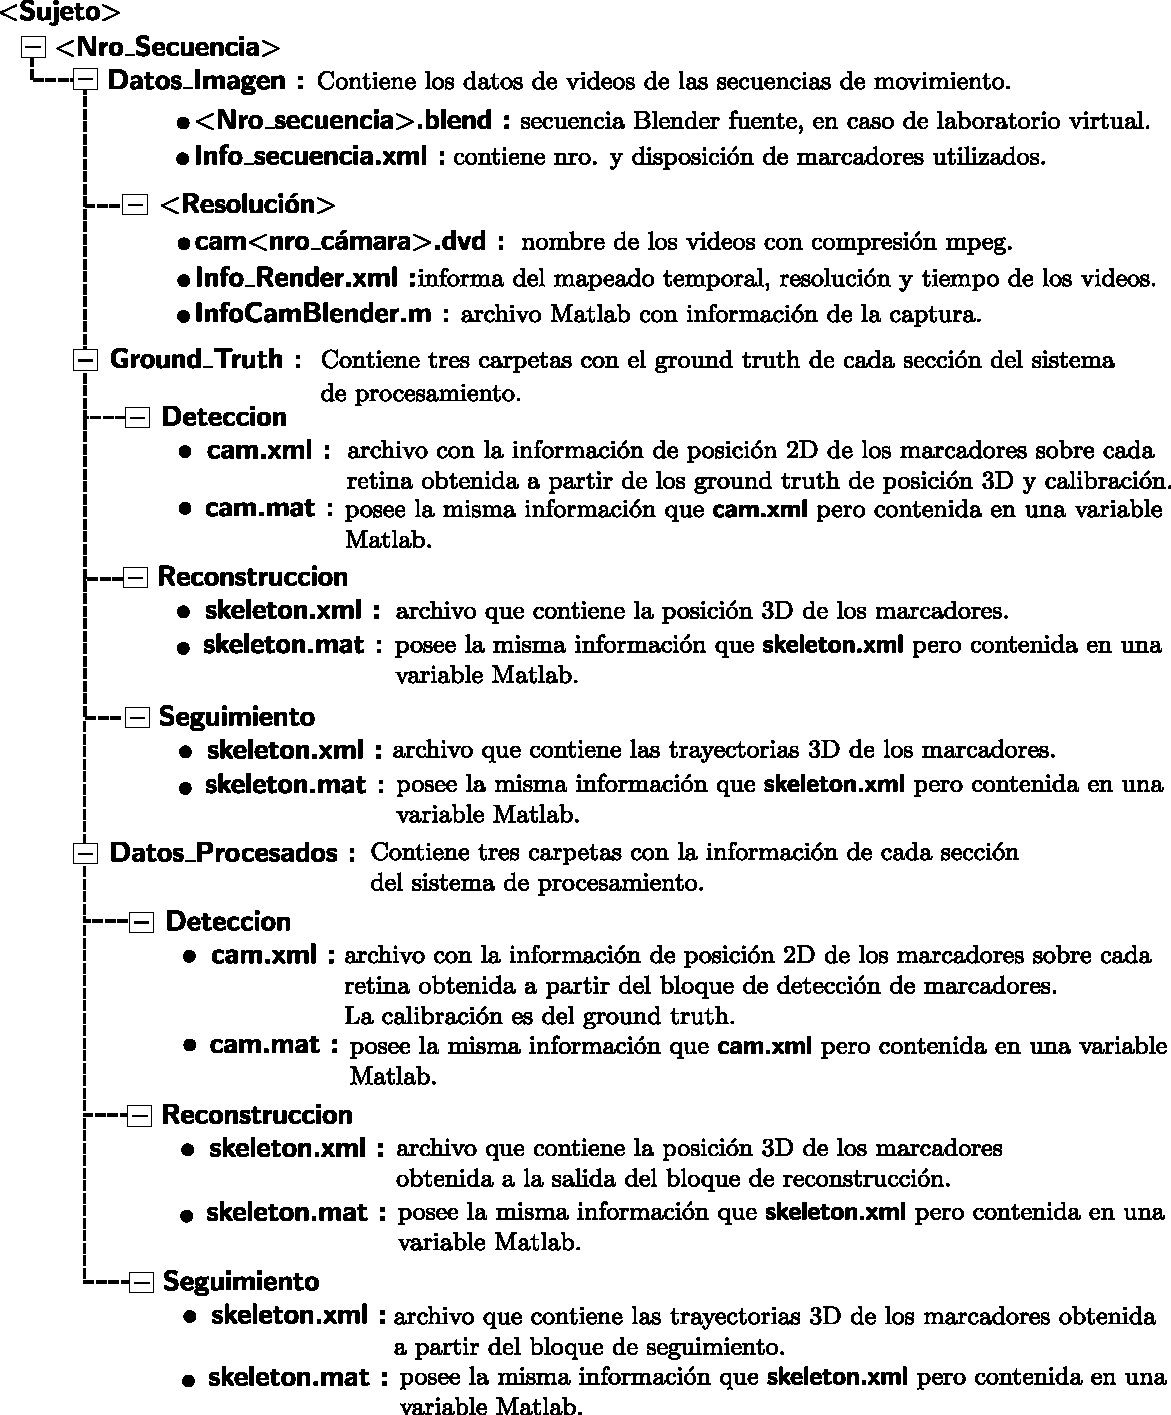
\includegraphics[scale=0.695]{img/Base_Datos/Estructura_directorios.pdf}
\caption{Estructura de directorios para almacenar información de capturas.}
\label{Estructura_directorios}
\end{figure}


\begin{figure}[ht!]
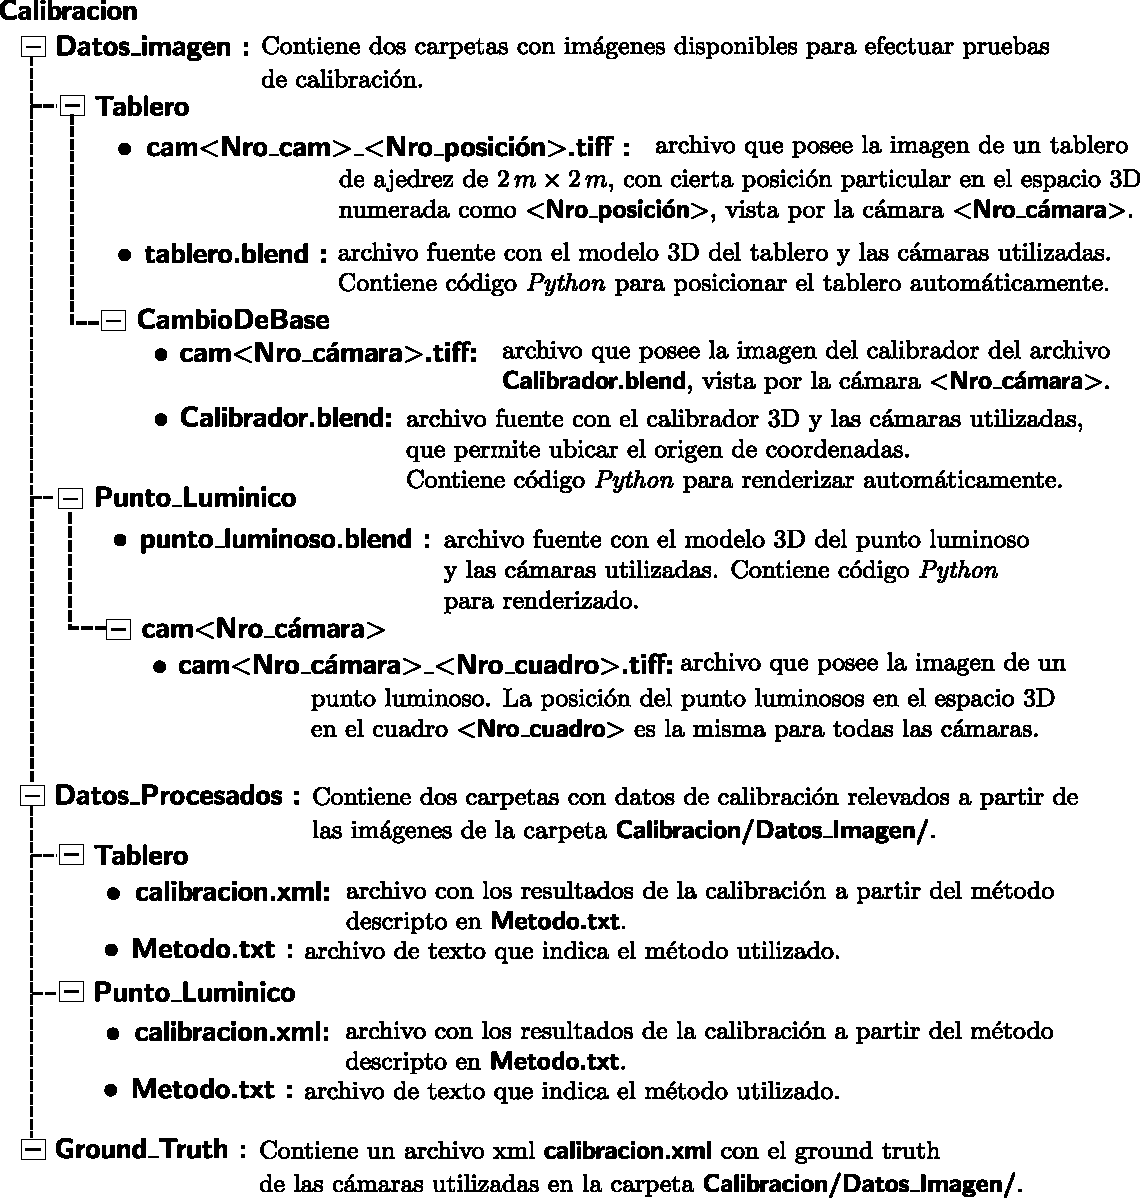
\includegraphics[scale=0.695]{img/Base_Datos/Estructura_directorios2.pdf}
\caption{Estructura de directorios para almacenar información de calibración.}
\label{Estructura_directorios2}
\end{figure}



Básicamente se tiene la información de cada secuencia de un sujeto separada en tres niveles: los datos de video, la información obtenida con los algoritmos al procesar los datos de video y por último,  si se encuentra disponible, la información de ground truth del mismo.


En el caso de secuencias sintéticas, fuera del entorno virtual se debe contar con los videos de la secuencia y el ground truth tanto de la calibración como del movimiento del esqueleto. 
La generación y ubicación de los videos en la estructura se efectúa mediante el código  \texttt{render.py}, luego la exportación del ground truth de la calibración a un archivo .m de \textit{Matlab}, se efectúa a través de \texttt{obtener\_InfoCam.py}. Ambos códigos fueron implementados de manera independiente del número y disposición de las cámaras. El movimiento del esqueleto es exportado a un archivo BVH a partir de las herramientas disponibles en \textit{Blender}.


Una vez finalizada la exportación de información del entorno \textit{Blender} se implementaron rutinas de \textit{Matlab} que permiten gestionar y ordenar dicha información en las secciones correspondientes de la estructura de directorios, conociendo el nombre del sujeto y el número de secuencia que distingue el movimiento desarrollado. 

Armado el laboratorio y ubicadas las cámaras para la captura de varias secuencias, el proceso de calibración y almacenamiento de sus variables se efectúa una sola vez. Por lo que ambas estructuras de directorios, la de información de captura y la de información de calibración,  se pueden almacenar en una única carpeta que identifique la configuración del laboratorio particular.  

\section{Estructura de datos.}
\label{section_Estructura_de_datos}
Para poder trabajar a lo largo de todo el sistema de procesamiento se debe contar con una estructura de datos que mantenga y soporte toda la información de interés a lo largo proceso. También es deseable que los procesos utilicen dicha estructura sin quedar condicionados a futuras modificaciones de la misma, esta independencia requiere la existencia de funciones de acceso de entrada y salida a la estructura.  


Con este fin se ha diseñado e implementado las estructuras de datos de las figuras \ref{img_estructura_skeleton} y \ref{img_estructura_cam}.
Las mismas permiten almacenar tanto la información de ground truth como la generada a la hora de  trabajar en las etapas de análisis de video. Se han implementado funciones de acceso de entrada y salida en \textit{Matlab}, así como varias herramientas de gestión que permiten entre otras cosas inicializar las estructuras, obtener o modificar cualquier parámetro, efectuar exportación e importación a xml y visualizar la información de manera interactiva generando para ello gráficas 2D o 3D. 


\begin{figure}[ht!]
   \hspace{-1.2cm}
   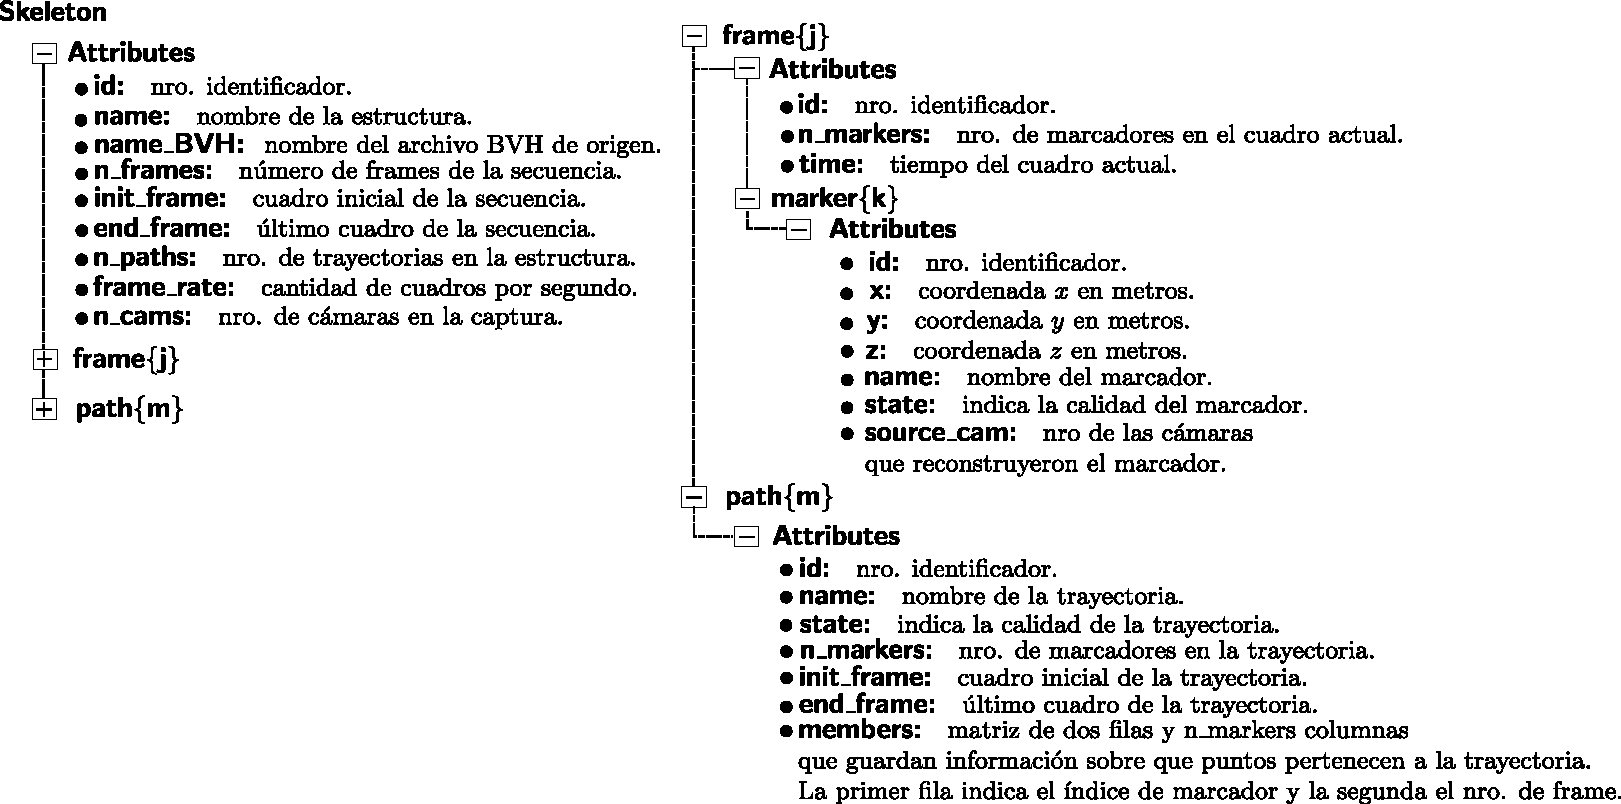
\includegraphics[scale=0.6]{img/Base_Datos/Estructura_datos_skeleton.pdf}
   \caption{Estructura de datos para esqueletos.}  
   \label{img_estructura_skeleton} 
 \end{figure} 

\begin{figure}[ht!]
   \hspace{-1.2cm}
   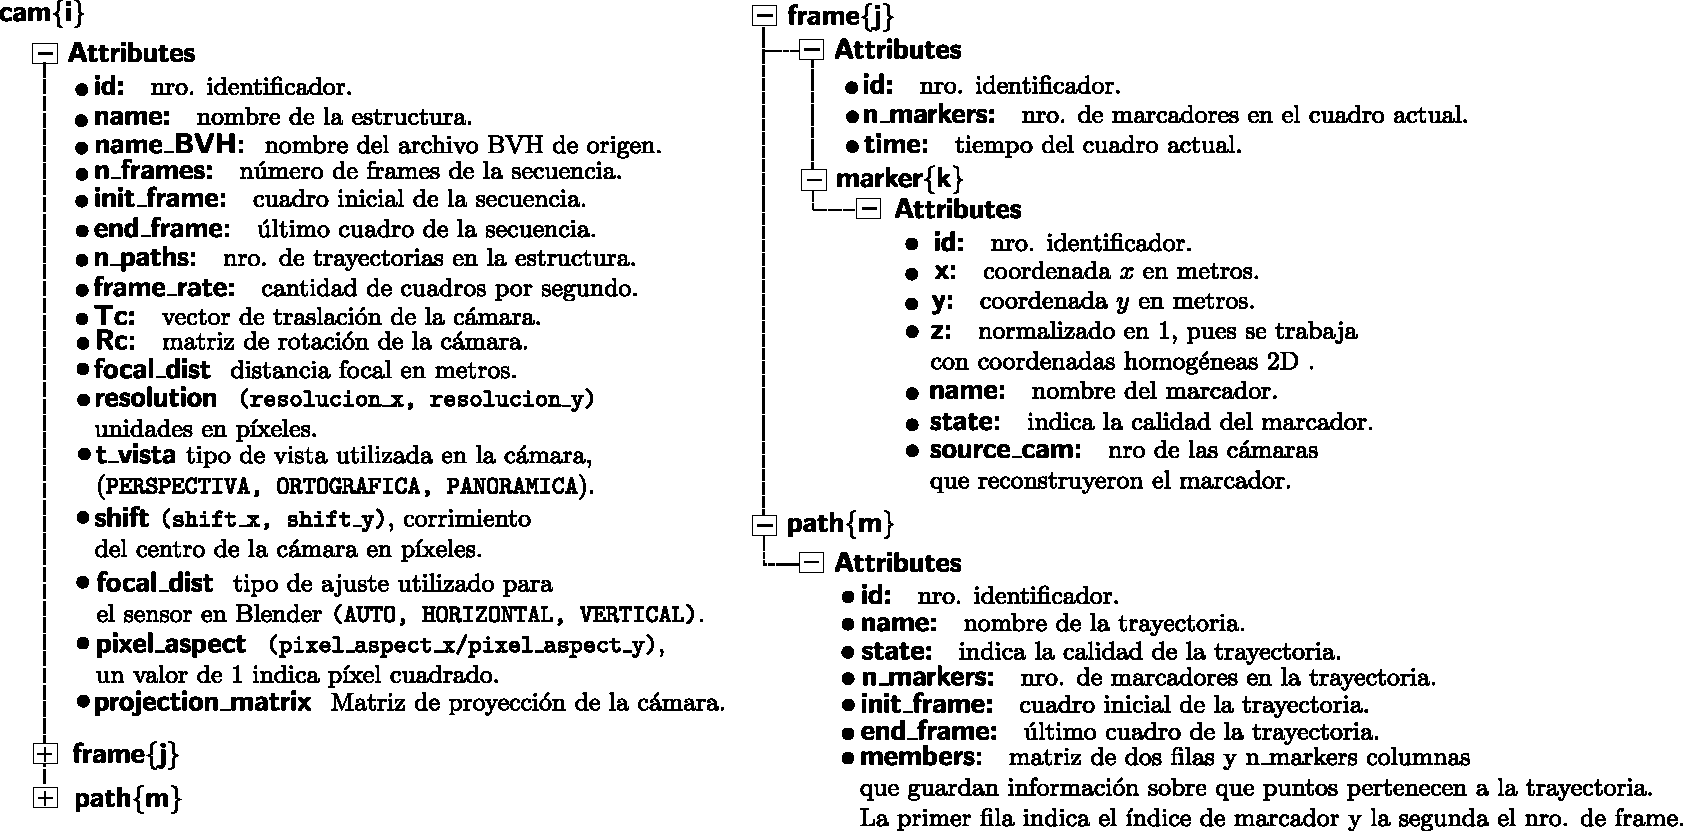
\includegraphics[scale=0.6]{img/Base_Datos/Estructura_datos_cam.pdf}
   \caption{Estructura de datos para cámaras.}
   \label{img_estructura_cam}    
 \end{figure} 


Por ejemplo si se desea obtener una estructura para almacenar la información 3D del sujeto a lo largo del procesamiento, se inicializa una estructura \texttt{skeleton} a través de la función \texttt{init\_structs()}, donde se indica entre otros parámetros el número de cuadros y número de marcadores. 
A partir de este momento se tiene una variable de nombre \texttt{skeleton} como la mostrada en la Figura \ref{img_estructura_skeleton} con sus campos inicializados. Luego se dispone las funciones \texttt{set\_info()} y \texttt{get\_info()}, que permiten modificar o acceder respectivamente a cualquier campo de la estructura. Las funciones que modifican la estructura lo hacen de una manera coherente, es decir si por ejemplo se introducen las coordenadas de un marcador en un cierto cuadro, se incrementa automáticamente el atributo \texttt{n\_markers} en el cuadro respectivo.

Básicamente se tienen dos estructuras principales, una para almacenar información del esqueleto asociado al modelo y otra para almacenar la información de las cámaras con las que se efectúa la captura de video.

Cabe destacar que este tipo de estructura es útil tanto para una base de datos sintética como una base de datos real. 





\section{Resumen} 

Si bien se encontraron numerosas bases de datos para la marcha, todas ellas terminan siendo descartadas por no ajustarse completamente a las hipótesis bajo las cuales se trabaja en este proyecto. Deficiencias tales como la inadecuada cantidad o posición de las cámaras, condiciones del laboratorio que dificultan y en algunos casos imposibilitan, una correcta segmentación a partir de la información óptica. Y por último la ausencia o tamaño inadecuado de los marcadores, son los factores más importantes.


Salvando diferencias, el problema principal está en que no se tienen imágenes ópticas para trabajar con marcadores, en general se tiende a trabajar sobre el cuerpo completo, y se contrasta el procesamiento con datos Mocap relevados con sistemas infrarrojos. Por otro lado esto último genera una rica fuente de material de trayectorias de puntos 3D en distinto tipo de movimientos, sobre todo en formatos Mocap.



Estas consideraciones impulsaron la idea de recorrer el camino inverso, crear una base de datos sintética a partir del material Mocap disponible, para luego generar los videos en los cuales trabajar.  


De todas maneras cabe destacar que se genera un relevamiento de bases de datos para el movimiento humano, se profundiza en las características usuales que presentan dichas bases de datos y se logra reunir un conjunto de conceptos y herramientas necesarios para introducirnos en el tema. \\

% % % % % % % % % % % % % % % % % % % % % % % % % % % % % % % %


A la hora de configurar un laboratorio no solo hay que integrar las distintas variables, sino también cuidar que esta integración se gestione de manera compatible, de lo contrario se estaría desaprovechando el potencial de las secuencias generadas por el sistema de captura en cuanto al procesamiento posterior se trata, dificultando la tarea de obtención de datos a partir de las secuencias de video.
En esta sección se logra tratar algunos parámetros claves y se discute las relaciones que estos deben tener para generar capturas de movimiento con información óptica basada en marcadores de bueno calidad.


A continuación se enumeran consideraciones de parámetros importantes para generar capturas en el caso de la marcha.

Es deseable para una buena resolución temporal poseer cámaras que permitan capturar 30 cuadros por segundo, con tiempos de obturación de al menos $1/2000\, s$, esto último permite evitar efectos de distorsión debidos a falta de nitidez. La resolución espacial de los datos en el procesamiento condiciona la resolución de la cámara. Se concluye que trabajando a 10 metros con resolución $1600\times600$ se obtienen incertidumbres de píxel de casi $1 ~cm $. 


El color de los  marcadores debe contrastar claramente con la vestimenta y el fondo del espacio de captura, se recomienda una forma esférica. En capturas con cámaras ubicadas a menos de 12 metros del movimiento a relevar, un tamaño aceptable para el marcadores es de $3\,cm$ de diámetro.

La vestimenta debe ser ajustada, para despreciar fluctuaciones en la posición de los marcadores y preferiblemente de igual color que el fondo.  

En cuanto a la iluminación, la misma debe ser uniforme, por ello si se utiliza iluminación artificial con focos puntuales es habitual colocar pantallas difusoras delante de los focos.

El espacio de captura debe contrastar con los marcadores, y sus dimensiones varían según el tipo de marcha a relevar. En caso de marcha rectilínea sobre una plataforma de $3\,m \times 5 \,m$ se encuentra que 4 son el mínimo número de cámaras que permiten relevar el movimiento de manera satisfactoria. Mientras  que en el caso de la marcha libre sobre una plataforma circular de $5\,m$ de diámetro, se recomienda la utilización de 8 cámaras. Una posible disposición de las mismas se muestra en la Figura \ref{img_espacio_capura}. \\
% % % % % % % % % % % % % % % % % % % %
% % % % % % % % % % % % % % % % % % % %

Al investigar los diferentes formatos de captura de movimiento (MoCap) disponibles en las distintas bases de datos relevadas, surge naturalmente el formato BVH como el propicio para importar la información de la captura de movimiento al entorno virtual y a \textit{Matlab}, su relativa sencillez y extendido uso facilitan sobremanera dicho pasaje. 

Se decide trabajar en este proyecto con las fuentes BVH de la base de datos \textit{MotionBuilder-friendly version} ofrecidas por \textit{cgspeed} \cite{cgspeed}, 
%\footnote{\textcolor{blue}{\underline{\url{https://sites.google.com/a/cgspeed.com/cgspeed/motion-capture}}}. Accedido 4-12-14},
 que provienen de las capturas de Carnegie Mellon University Motion Capture Database \cite{CMU}.
 %\footnote{\textcolor{blue}{\underline{\url{http://mocap.cs.cmu.edu/}}}. Accedido 30-11-14}. 
 Alguno de los factores que justifican esta elección son que C.M.U. dispone de un gran número de capturas de movimiento de acceso público, varias utilidades de software que permiten llevar a otros formatos y es utilizado ampliamente en el ámbito de la animación por computadora.
 
 Utilizando una suite de animación 3D gratuita y de código abierto como lo es \textit{Blender}, se genera un laboratorio de captura de movimiento virtual, donde logra obtenerse cinco secuencias sintéticas dentro de los cuales cuatro son movimientos de marcha y una de corrida, con sus respectivos videos.  Si bien las secuencias de video obtenidas son lo único necesario para el análisis posterior, al generar dichas secuencias a través de un entorno virtual controlado como lo es \textit{Blender}, se puede obtener la información exacta del ambiente de captura. Información de las cámaras, iluminación, colores, ruido, posición de los marcadores en cada cuadro, etc. Permitiendo contar con un ground truth tanto del movimiento como de la calibración de las cámaras, sobre el cual validar los algoritmos en cada etapa del sistema de procesamiento. Esto último también permite obtener un benchmark de algoritmos, sumamente importante en futuros trabajos sobre el sistema. 
 
   
\textit{Blender} cuenta con una interfaz de programación de aplicaciones flexible, que permite extender su funcionalidad a través de programas en Python. Con el objetivo de automatizar varias etapas en el desarrollo de nuevas secuencias, así como gestionar la exportación de información desde \textit{Blender} a otros lenguajes, se han creado múltiples scripts. En particular se posee un programa Python que automatiza la extracción de parámetros de interés hacía un archivo xml con cierta estructura particular ya definida en la base de datos. 


La estructura de datos implementada cuenta con lo necesario para mantener y dar soporte a la información de interés a lo largo del proyecto. Cabe destacar que también soporta información de secuencias reales.



Se logra implementar un prototipo de base de datos lo suficientemente general y útil para trabajar con sistemas de captura de movimiento basada en marcadores. Las características de las herramientas utilizadas permiten generar secuencias de movimiento sintéticas, con relativa facilidad. El potencial actual y la posible expansión de la base de datos permiten afirmar que la misma es una herramienta a tener en cuenta en futuros proyectos de captura de movimiento.

% % % % % % % % % % % % % % % % % % % % %